\chapter{Various}
\label{chapter:various}

\newcounter{various}
\setcounter{various}{0}
\stepcounter{various}

\section{Example \thevarious}
\stepcounter{various}

\begin{figure}[h]
	\begin{center}
		\scalebox{0.5}{
			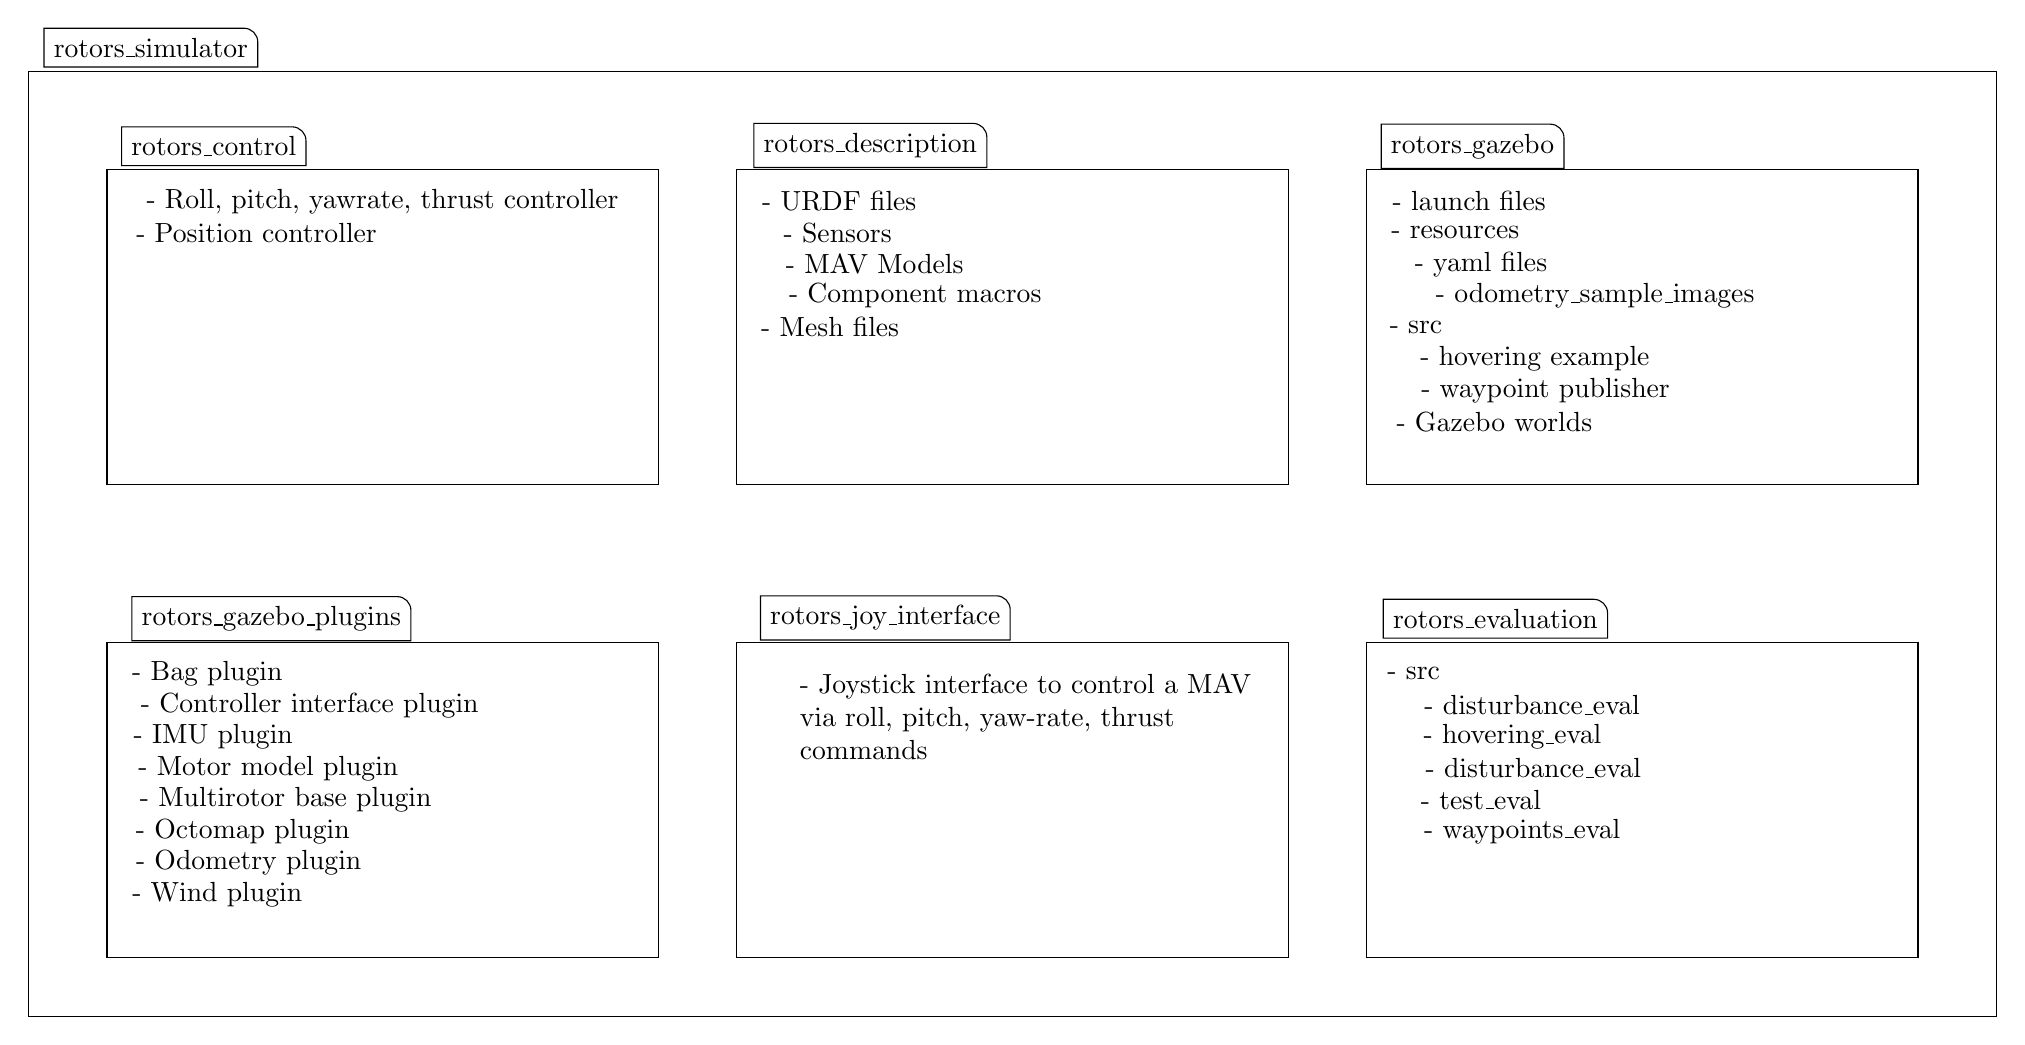
\begin{tikzpicture}
			
			%Package comments
			\node (Rotors Control) at (0,0) [draw, rectangle, minimum height=4cm, minimum 
			width=7cm, text centered]{};
			\draw node at (-2.1435,2.3)[
			append after command={[rounded corners=0pt](b.west)|-(b.north)},
			append after command={[rounded corners=5pt](b.north)-|(b.east)},
			append after command={[rounded corners=0pt](b.east)|-(b.south)},
			append after command={[rounded corners=0pt](b.south)-|(b.west)}] 
			(b) {rotors\_control};
			
			%Writing in the box
			\node at (0,1.6) [text centered]{- Roll, pitch, yawrate, thrust controller};
			\node at (-1.6,1.2) [text centered]{- Position controller};
			
			%Second block
			\node (Rotors Description) at (8,0) [draw, rectangle, minimum height=4cm, minimum 
			width=7cm, text centered]{};
			\draw node at (6.195,2.31)[
			append after command={[rounded corners=0pt](b.west)|-(b.north)},
			append after command={[rounded corners=5pt](b.north)-|(b.east)},
			append after command={[rounded corners=0pt](b.east)|-(b.south)},
			append after command={[rounded corners=0pt](b.south)-|(b.west)}] 
			(b) {rotors\_description};
			
			%Writing in the box
			\node at (5.8,1.6) [text centered]{- URDF files};
			\node at (5.78,1.2) [text centered]{- Sensors};
			\node at (6.25,0.8) [text centered]{- MAV Models};
			\node at (6.765,0.4) [text centered]{- Component macros};
			\node at (5.685,0) [text centered]{- Mesh files};
			
			%Third block
			\node (Rotors Gazebo) at (16,0) [draw, rectangle, minimum height=4cm, minimum 
			width=7cm, text centered]{};
			\draw node at (13.8435,2.3)[
			append after command={[rounded corners=0pt](b.west)|-(b.north)},
			append after command={[rounded corners=5pt](b.north)-|(b.east)},
			append after command={[rounded corners=0pt](b.east)|-(b.south)},
			append after command={[rounded corners=0pt](b.south)-|(b.west)}] 
			(b) {rotors\_gazebo};
			
			%Writing in the box
			\node at (13.8,1.6) [text centered]{- launch files};
			\node at (13.625,1.2) [text centered]{- resources};
			\node at (13.95,0.8) [text centered]{- yaml files};
			\node at (15.4,0.4) [text centered]{- odometry\_sample\_images};
			\node at (13.125,0.0) [text centered]{- src};
			\node at (14.635,-0.4) [text centered]{- hovering example};
			\node at (14.77,-0.8) [text centered]{- waypoint publisher};
			\node at (14.12,-1.2) [text centered]{- Gazebo worlds};
			
			%Fourth block
			\node (Rotors Control) at (0,-6) [draw, rectangle, minimum height=4cm, minimum 
			width=7cm, text centered]{};
			\draw node at (-1.4115,-3.7)[
			append after command={[rounded corners=0pt](b.west)|-(b.north)},
			append after command={[rounded corners=5pt](b.north)-|(b.east)},
			append after command={[rounded corners=0pt](b.east)|-(b.south)},
			append after command={[rounded corners=0pt](b.south)-|(b.west)}] 
			(b) {rotors\_gazebo\_plugins};
			
			%Writing in the box
			\node at (-2.225,-4.4) [text centered]{- Bag plugin};
			\node at (-0.925,-4.8) [text centered]{- Controller interface plugin};
			\node at (-2.15,-5.2) [text centered]{- IMU plugin};
			\node at (-1.45,-5.6) [text centered]{- Motor model plugin};
			\node at (-1.23,-6.0) [text centered]{- Multirotor base plugin};
			\node at (-1.775,-6.4) [text centered]{- Octomap plugin};
			\node at (-1.7,-6.8) [text centered]{- Odometry plugin};
			\node at (-2.1,-7.2) [text centered]{- Wind plugin};
			
			
			%Fifth block
			\node (Rotors Joy Interface) at (8,-6) [draw, rectangle, minimum height=4cm, minimum 
			width=7cm, text centered]{};
			\draw node at (6.385,-3.69)[
			append after command={[rounded corners=0pt](b.west)|-(b.north)},
			append after command={[rounded corners=5pt](b.north)-|(b.east)},
			append after command={[rounded corners=0pt](b.east)|-(b.south)},
			append after command={[rounded corners=0pt](b.south)-|(b.west)}] 
			(b) {rotors\_joy\_interface};
			
			%Writing in the box
			\node at (11.45,-4.95) [text width=35em]{- Joystick interface to control a MAV\\via 
			roll, pitch, yaw-rate, thrust\\commands};
			
			%Sixth block
			\node (Rotors Evaluation) at (16,-6) [draw, rectangle, minimum height=4cm, minimum 
			width=7cm, text centered]{};
			\draw node at (14.1335,-3.70)[
			append after command={[rounded corners=0pt](b.west)|-(b.north)},
			append after command={[rounded corners=5pt](b.north)-|(b.east)},
			append after command={[rounded corners=0pt](b.east)|-(b.south)},
			append after command={[rounded corners=0pt](b.south)-|(b.west)}] 
			(b) {rotors\_evaluation};
			
			%Writing in the box
			\node at (13.095,-4.4) [text centered]{- src};
			\node at (14.6,-4.8) [text centered]{- disturbance\_eval};
			\node at (14.35,-5.2) [text centered]{- hovering\_eval};
			\node at (14.615,-5.6) [text centered]{- disturbance\_eval};
			\node at (13.95,-6.0) [text centered]{- test\_eval};
			\node at (14.475,-6.4) [text centered]{- waypoints\_eval};
			
			%Container
			\node (container) at (8,-2.75) [draw, rectangle, minimum height=12cm, minimum 
			width=25cm]{};
			\draw node at (-2.9421,3.5525)[
			append after command={[rounded corners=0pt](b.west)|-(b.north)},
			append after command={[rounded corners=5pt](b.north)-|(b.east)},
			append after command={[rounded corners=0pt](b.east)|-(b.south)},
			append after command={[rounded corners=0pt](b.south)-|(b.west)}] 
			(b) {rotors\_simulator};
			
			\end{tikzpicture}
		}
	\end{center}

\end{figure}

\section{Example \thevarious}
\stepcounter{various}

\begin{figure}[h]
	\begin{center}
		\scalebox{0.8}{
		
\begin{tikzpicture}[blend group=screen]
		\fill[red!90!black]   ( 90:.6) circle (1.5);
		\fill[green!80!black] (210:.6) circle (1.5);
		\fill[blue!90!black] (330:.6) circle (1.5);
		\end{tikzpicture}
	}
	\end{center}
\end{figure}

\newpage


\section{Example \thevarious}
\stepcounter{various}

\begin{figure}[h]
	\begin{center}
		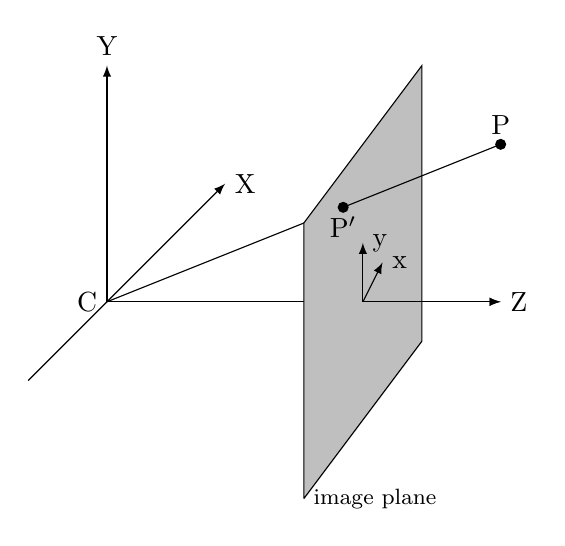
\begin{tikzpicture}
		
		\draw[-latex] (0,0) node[anchor=east]{C} -- (5,0) node[anchor=west] {Z};
		\draw[-latex] (0,0) -- (0,3) node[anchor=south] {Y};
		\draw[-latex] (-1.0,-1.0) -- (1.5,1.5) node[anchor=west] {X};
		\draw (0,0) -- (3,1.2);
		\filldraw[fill=lightgray] (2.5,-2.5) -- (2.5,1) --  (4,3) -- (4,-0.5) -- (2.5,-2.5);
		\draw[-latex] (3.25,0) -- (3.25,0.75) node[anchor=west] {y};
		\draw[-latex] (3.25,0) -- (3.5,0.5) node[anchor=west] {x};
		\draw[-latex] (3.25,0) -- (5,0);
		\draw (3,1.2) -- (5,2);
		\fill (5,2) circle[radius=2pt] node[anchor=south] {P};
		\fill (3,1.2) circle[radius=2pt] node[anchor=north] {P$'$};
		\draw (2.5,-2.5) node[anchor=west, font=\footnotesize] {image plane};
		
		\end{tikzpicture}
	\end{center}
	
\end{figure}


\section{Example \thevarious}
\stepcounter{various}

\begin{figure}[h]
	\begin{center}
		\begin{tikzpicture}
		
		%Reference system
		\draw[dashed] (0,0) coordinate -- (0,3) coordinate;
		\draw[-latex] (0,3) coordinate -- (0,4.2) coordinate node[above 
		left]{$Z_\mathrm{ECI}\,Z_\mathrm{ECEF}$};
		\draw (0,3.25) node[above left]{North Pole};
		\draw[dashed] (0,0) coordinate -- (-2.45,-2.45) coordinate;
		\draw[-latex] (-2.45,-2.45) coordinate -- (-3.5,-3.5) coordinate node [below 
		left]{$X_\mathrm{ECEF}$};
		\draw[-latex, dashed] (0,0) coordinate -- (-5,-1) coordinate node[left]{$X_\mathrm{ECI}$};
		\draw (-2.3,-3.6) node[right, text width=3cm]{Greenwich Meridian};
		\draw[dashed] (0,0) coordinate -- (4,0);
		\draw[-latex] (4,0) coordinate -- (5,0) coordinate node [above right]{$Y_\mathrm{ECEF}$};
		\draw[-latex, dashed] (0,0) coordinate -- (5.0,-1) coordinate node[right]{$Y_\mathrm{ECI}$};
		\draw (-4.8,-0.6) node[above, text width=2cm]{Vernal equinox};
		
		%First line and angle
		\draw[-] (-1,-1) coordinate (a) -- (0,0) coordinate (b) -- (2.17,-1.26) coordinate (c)
		pic[right,"$l$", draw, -latex, angle eccentricity=1.2, angle radius=1cm]{angle=a--b--c};
		
		%Second line and angle
		\draw[dotted] (2.17,-1.26) coordinate (d) -- (0.70,-0.40) coordinate (e) -- (2.17,1.77) 
		coordinate (f)
		pic["$\bar{\phi}$", draw, -latex, angle eccentricity=0.7, angle 
		radius=0.8cm]{angle=d--e--f};
		
		%Third line and angle
		\draw[-] (2.17,-1.26) coordinate (g) -- (0,0) coordinate (h) -- (2.17,1.77) coordinate (i)
		pic["$\Psi$", draw, blue, -latex, angle eccentricity=0.9, angle 
		radius=2.1cm]{angle=g--h--i};
		
		%Fourth line and angle
		\coordinate (l) at (-5,-1);
		\coordinate (m) at (0,0); 
		\coordinate (n) at (-3.5,-3.5);
		\draw pic["$l_o+\omega_E\,t$", draw, -latex, angle eccentricity=1.2, angle 
		radius=4.2cm]{angle=l--m--n};
		
		%Horizontal axis
		\draw (0,0) ellipse (4cm and 3cm);
		
		%Vertical ellipse
		\draw[dashed] (4,0) arc (0:180:4cm and 1.5cm);
		\draw (-4,0) arc (180:360:4cm and 1.5cm);
		
		%Arcs
		\draw[] (0,3) arc (100:199.5:4cm and 3cm);
		\draw (0,3) arc (90:0):3cm and 4cm);
		
		%Z-axis dashed
		\draw[dashed] (0,0) coordinate -- (0,-3) coordinate;
		\draw (0,-3) coordinate -- (0,-4) coordinate;
		
		%Reference system origin
		\draw (0,0) coordinate node[above left]{$O$};
		\draw[-, red] (0,0) coordinate -- (2.17,1.77) coordinate;
		\draw (2.2,1.5) coordinate node[above right]{$P$};
		\draw[dashed] (2.17,-1.26) coordinate -- (2.17,1.77) coordinate;
		
		%Second reference system
		\draw[-latex,line width=1.25pt] (2.17,1.77) coordinate -- (3.17,3.24) coordinate 
		node[above]{$-Z_v$};
		\draw[-latex,line width=1.25pt] (2.17,1.77) coordinate -- (1,3.2) coordinate 
		node[above]{$X_v$};
		\draw[-latex,line width=1.25pt] (2.17,1.77) coordinate -- (2.17,2.87) coordinate 
		node[above]{$Y_v$};
		
		\end{tikzpicture}
	\end{center}
	
\end{figure}

\newpage


\section{Example \thevarious}
\stepcounter{various}

\begin{figure}[h]
	\begin{center}
		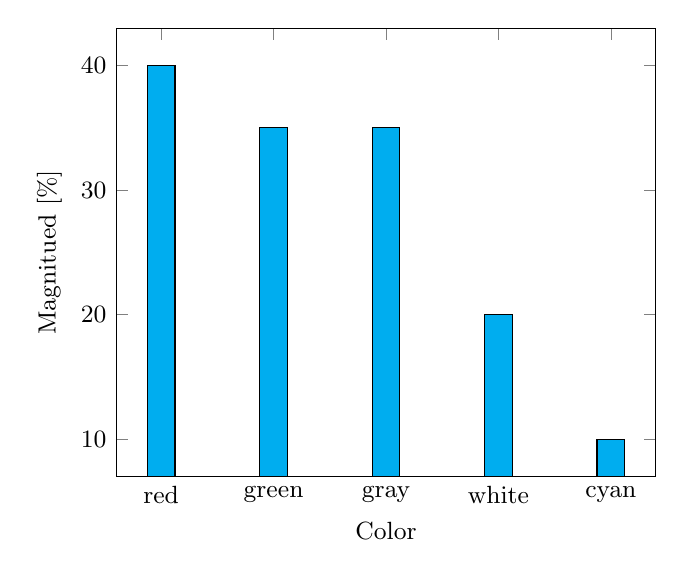
\begin{tikzpicture}[font=\small]
		
		%Histogram
		\begin{axis}[
		symbolic x coords={red, green, gray, white, cyan},
		ylabel = {Magnitued [$\%$]},
		xlabel = {Color},
		xtick=data
		]
		\addplot[ybar,draw=black, fill=cyan] coordinates {
			(red,  40)
			(green,  35)
			(gray, 35)
			(white, 20)
			(cyan,  10)
		};
		\end{axis}
		
		\end{tikzpicture}
	\end{center}
	
\end{figure}


\section{Example \thevarious}
\stepcounter{various}

\begin{figure}[h]
	\begin{center}
		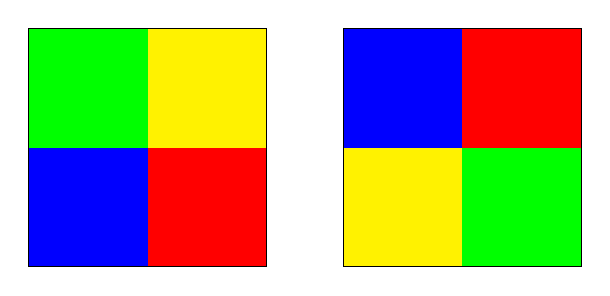
\begin{tikzpicture}
		
		%First squre
		\node (square) at (-2,0) [rectangle, draw, minimum width=3cm, minimum height=3cm, text 
		centered, line width=1.25pt]{};
		
		%Square divider
		\node (firstLine) at (-2.75, 0.75) [rectangle, fill=green, minimum width=1.5cm, minimum 
		height=1.5cm, text centered]{};
		\node (secondLine) at (-1.25, 0.75) [rectangle, fill=yellow, minimum width=1.5cm, minimum 
		height=1.5cm, text centered]{};
		\node (thirdLine) at (-2.75, -0.75) [rectangle, fill=blue, minimum width=1.5cm, minimum 
		height=1.5cm, text centered]{};
		\node (fourthLine) at (-1.25, -0.75) [rectangle, fill=red, minimum width=1.5cm, minimum 
		height=1.5cm, text centered]{};
		
		%Second squre
		\node (square2) at (2,0) [rectangle, draw, minimum width=3cm, minimum height=3cm, text 
		centered, line width=1.25pt]{};
		
		%Square divider
		\node (firstLine1) at (2.75, 0.75) [rectangle, fill=red, minimum width=1.5cm, minimum 
		height=1.5cm, text centered]{};
		\node (secondLine1) at (1.25, 0.75) [rectangle, fill=blue, minimum width=1.5cm, minimum 
		height=1.5cm, text centered]{};
		\node (thirdLine1) at (2.75, -0.75) [rectangle, fill=green, minimum width=1.5cm, minimum 
		height=1.5cm, text centered]{};
		\node (fourthLine1) at (1.25, -0.75) [rectangle, fill=yellow, minimum width=1.5cm, minimum 
		height=1.5cm, text centered]{};
		
		\end{tikzpicture}
	\end{center}
	
\end{figure}



\section{Example \thevarious}
\stepcounter{various}

\begin{figure}[h]
	\begin{center}
		\scalebox{0.8}{
		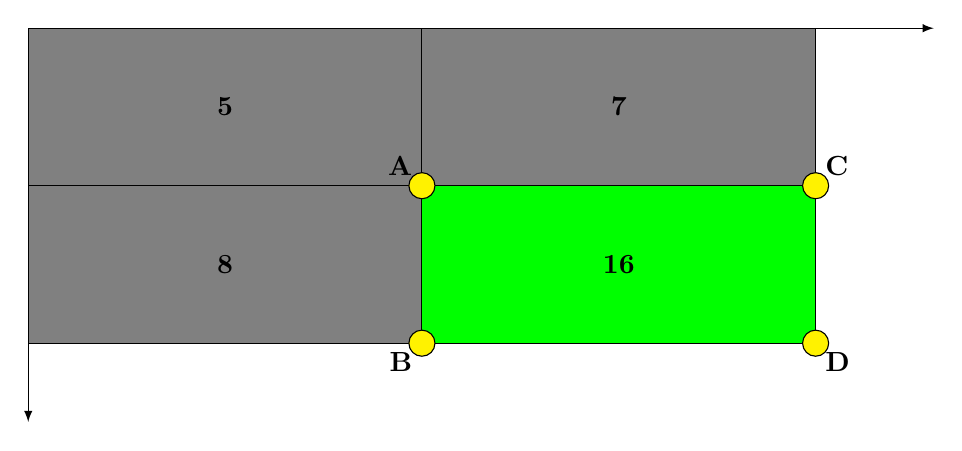
\begin{tikzpicture}
		
		%Squares
		\node (firstSquare) at (-5,5) [rectangle, draw, text centered, text width=6em, minimum 
		width=5cm, minimum height=2cm, fill=gray] {\textbf{5}};
		\node (secondSquare) at (0,5) [rectangle, draw, text centered, text width=6em, minimum 
		width=5cm, minimum height=2cm, fill=gray] {\textbf{7}};
		\node (thirdSquare) at (-5,3) [rectangle, draw, text centered, text width=6em, minimum 
		width=5cm, minimum height=2cm, fill=gray] {\textbf{8}};
		\node (fourthSquare) at (0,3) [rectangle, draw, text centered, text width=6em, minimum 
		width=5cm, minimum height=2cm, fill=green] {\textbf{16}};
		
		%Circles
		\node (firstCircle) at (-2.5,4) [circle, draw, text centered, minimum size=0.2cm, 
		fill=yellow]{};
		\node (secondCircle) at (-2.5,2) [circle, draw, text centered, minimum size=0.2cm, 
		fill=yellow]{};
		\node (thirdCircle) at (2.5,4) [circle, draw, text centered, minimum size=0.2cm, 
		fill=yellow]{};
		\node (fourthCircle) at (2.5,2) [circle, draw, text centered, minimum size=0.2cm, 
		fill=yellow]{};
		
		%Axes
		\draw[-latex] (-7.5,6) coordinate -- (4,6) coordinate;
		\draw[-latex] (-7.5,6) coordinate -- (-7.5,1) coordinate;
		
		%Letters
		\draw (-2.5, 4) coordinate node[above left]{\textbf{A}};
		\draw (2.5, 4) coordinate node[above right]{\textbf{C}};
		\draw (-2.5, 2) coordinate node[below left]{\textbf{B}};
		\draw (2.5, 2) coordinate node[below right]{\textbf{D}};
		
		\end{tikzpicture}
	}
	\end{center}
	
\end{figure}

\newpage

\section{Example \thevarious}
\stepcounter{various}

\begin{figure}[h]
	\begin{center}
		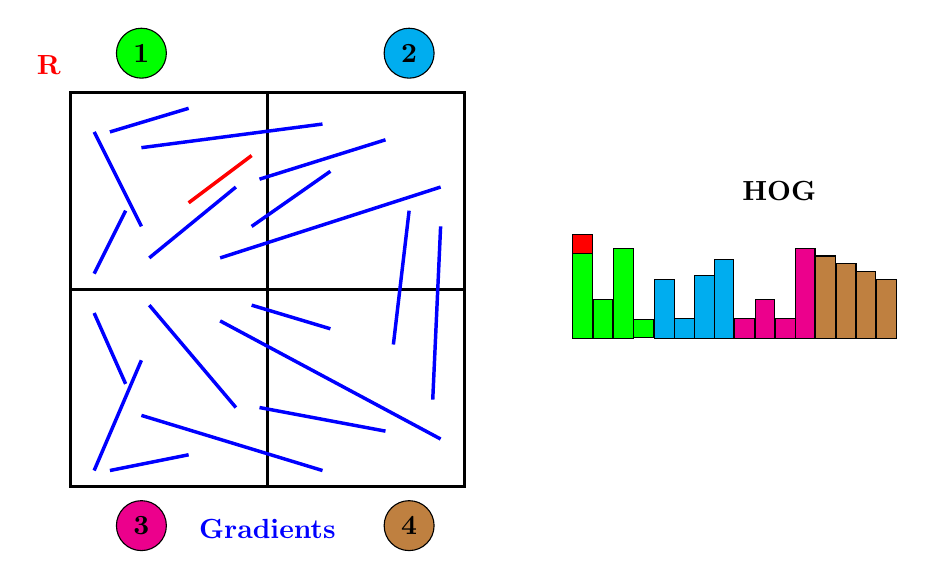
\begin{tikzpicture}
		
		%First squre
		\node (square) at (-5,0) [rectangle, draw, minimum width=5cm, minimum height=5cm, text 
		centered, line width=1.25pt]{};
		
		%Square divider
		\draw[-, line width=1.25pt] (-5,2.5) coordinate -- (-5, -2.5) coordinate;
		\draw[-, line width=1.25pt] (-7.5,0) coordinate -- (-2.5,0);
		
		%Lines
		\draw[-, blue, line width=1.25pt] (-7.2,0.2) coordinate -- (-6.8,1.0) coordinate;
		\draw[-, blue, line width=1.25pt] (-6.5, 0.4) coordinate -- (-5.4, 1.3) coordinate;
		\draw[-, blue, line width=1.25pt] (-6.6, 0.8) coordinate -- (-7.2, 2.0) coordinate;
		\draw[-, blue, line width=1.25pt] (-5.6, 0.4) coordinate -- (-2.8, 1.3) coordinate;
		\draw[-, blue, line width=1.25pt] (-5.2, 0.8) coordinate -- (-4.2, 1.5) coordinate;
		\draw[-, blue, line width=1.25pt] (-5.1, 1.4) coordinate -- (-3.5, 1.9) coordinate;
		\draw[-, blue, line width=1.25pt] (-7.0, 2.0) coordinate -- (-6.0, 2.3) coordinate;
		\draw[-, blue, line width=1.25pt] (-6.6, 1.8) coordinate -- (-4.3, 2.1) coordinate;
		
		\draw[-, blue, line width=1.25pt] (-7.2,-0.3) coordinate -- (-6.8, -1.2) coordinate;
		\draw[-, blue, line width=1.25pt] (-6.5, -0.2) coordinate -- (-5.4, -1.5) coordinate;
		\draw[-, blue, line width=1.25pt] (-6.6, -0.9) coordinate -- (-7.2, -2.3) coordinate;
		\draw[-, blue, line width=1.25pt] (-5.6, -0.4) coordinate -- (-2.8, -1.9) coordinate;
		\draw[-, blue, line width=1.25pt] (-5.2, -0.2) coordinate -- (-4.2, -0.5) coordinate;
		\draw[-, blue, line width=1.25pt] (-5.1, -1.5) coordinate -- (-3.5, -1.8) coordinate;
		\draw[-, blue, line width=1.25pt] (-7.0, -2.3) coordinate -- (-6.0, -2.1) coordinate;
		\draw[-, blue, line width=1.25pt] (-6.6, -1.6) coordinate -- (-4.3, -2.3) coordinate;
		
		\draw[-, blue, line width=1.25pt] (-2.8, 0.8) coordinate -- (-2.9, -1.4) coordinate;
		\draw[-, blue, line width=1.25pt] (-3.2, 1.0) coordinate -- (-3.4, -0.7) coordinate;
		
		\draw[-, red, line width=1.25pt] (-6.0, 1.1) coordinate -- (-5.2, 1.7) coordinate;
		
		%Histogram
		\node (rectangle1) at (-1,-0.05) [rectangle, draw, minimum width=0.25cm, fill=green, 
		minimum height=1.15cm, text centered]{};
		\node (rectangle) at (-1,0.575) [rectangle, draw, minimum width=0.25cm, fill=red, minimum 
		height=0.15cm, text centered]{};
		\node (rectangle2) at (-0.74,-0.375) [rectangle, draw, fill=green, minimum width=0.25cm, 
		minimum height=0.5cm, text centered]{};
		\node (rectangle3) at (-0.48,-0.05) [rectangle, draw, fill=green, minimum width=0.25cm, 
		minimum height=1.15cm, text centered]{};
		\node (rectangle4) at (-0.22,-0.497) [rectangle, draw, fill=green, minimum width=0.25cm, 
		minimum height=0.15cm, text centered]{};
		\node (rectangle5) at (0.04,-0.25) [rectangle, draw, fill=cyan, minimum width=0.25cm, 
		minimum height=0.75cm, text centered]{};
		\node (rectangle6) at (0.30,-0.497) [rectangle, draw, fill=cyan, minimum width=0.25cm, 
		minimum height=0.25cm, text centered]{};
		\node (rectangle7) at (0.55,-0.225) [rectangle, draw, fill=cyan, minimum width=0.25cm, 
		minimum height=0.80cm, text centered]{};
		\node (rectangle8) at (0.80,-0.125) [rectangle, draw, fill=cyan, minimum width=0.25cm, 
		minimum height=1.00cm, text centered]{};
		\node (rectangle9) at (1.06,-0.497) [rectangle, draw, minimum width=0.25cm, fill=magenta, 
		minimum height=0.25cm, text centered]{};
		\node (rectangle10) at (1.32,-0.375) [rectangle, draw, fill=magenta, minimum width=0.25cm, 
		minimum height=0.5cm, text centered]{};
		\node (rectangle11) at (1.58,-0.497) [rectangle, draw, fill=magenta, minimum width=0.25cm, 
		minimum height=0.25cm, text centered]{};
		\node (rectangle12) at (1.83,-0.05) [rectangle, draw, fill=magenta, minimum width=0.25cm, 
		minimum height=1.15cm, text centered]{};
		\node (rectangle13) at (2.09,-0.1) [rectangle, draw, fill=brown, minimum width=0.25cm, 
		minimum height=1.05cm, text centered]{};
		\node (rectangle14) at (2.35,-0.15) [rectangle, draw, fill=brown, minimum width=0.25cm, 
		minimum height=0.95cm, text centered]{};
		\node (rectangle15) at (2.60,-0.2) [rectangle, draw, fill=brown, minimum width=0.25cm, 
		minimum height=0.85cm, text centered]{};
		\node (rectangle16) at (2.86,-0.25) [rectangle, draw, fill=brown, minimum width=0.25cm, 
		minimum height=0.75cm, text centered]{};
		
		%Names
		\draw (1.5, 1.0) coordinate node[above]{\textbf{HOG}};
		\draw[blue] (-5,-2.8) coordinate node[below]{\textbf{Gradients}};
		\draw[red] (-7.5,2.6) node[above left]{\textbf{R}};
		
		%Circles
		\node (firstCircle) at (-6.6,3.0) [circle, draw, text centered, minimum size=0.2cm, 
		fill=green]{\textbf{1}};
		\node (secondCircle) at (-3.2,3.0) [circle, draw, text centered, minimum size=0.2cm, 
		fill=cyan]{\textbf{2}};
		\node (thirdCircle) at (-6.6,-3.0) [circle, draw, text centered, minimum size=0.2cm, 
		fill=magenta]{\textbf{3}};
		\node (fourthCircle) at (-3.2,-3.0) [circle, draw, text centered, minimum size=0.2cm, 
		fill=brown]{\textbf{4}};
		
		\end{tikzpicture}
	\end{center}
\end{figure}



\section{Example \thevarious}
\stepcounter{various}

\begin{figure}[h]
	\begin{center}
		\scalebox{0.9}{
		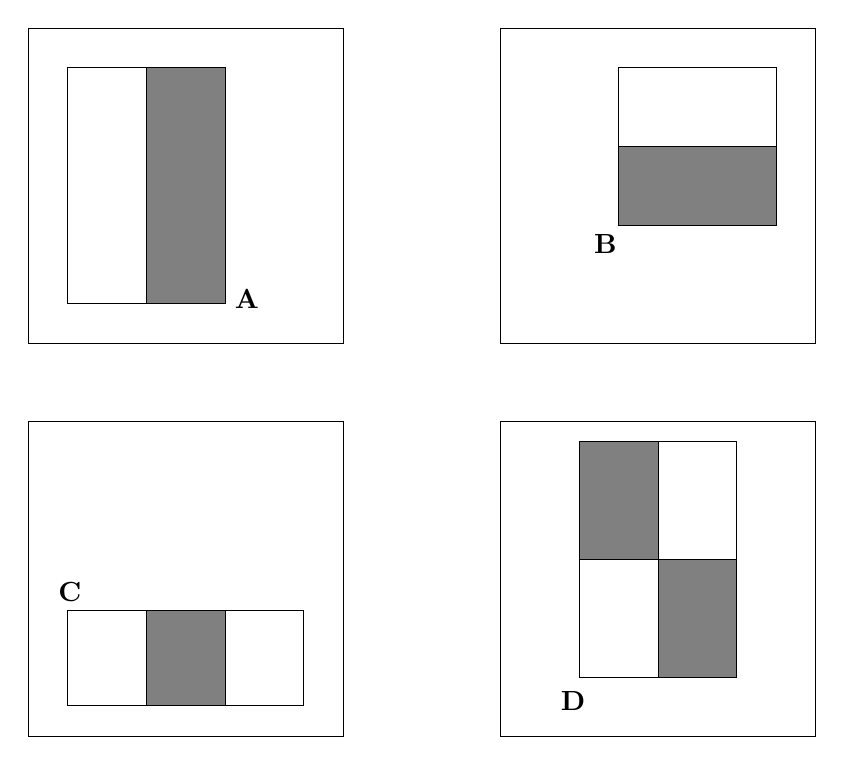
\begin{tikzpicture}
		
		%First square
		\node (firstSquare) at (-3,5) [rectangle, draw, text centered, minimum width=4cm, minimum 
		height=4cm]{};
		
		\node (firstSubSquare1) at (-4,5) [rectangle, draw, text centered, minimum width=1cm, 
		minimum height=3cm]{};
		\node (secondSubSquare1) at (-3,5) [rectangle, draw, text centered, minimum width=1cm, 
		minimum height=3cm, fill=gray]{};
		
		\draw (-2.5, 3.8) coordinate node[below right]{\textbf{A}};
		
		%Second square
		\node (secondSquare) at (3,5) [rectangle, draw, text centered, minimum width=4cm, minimum 
		height=4cm]{};
		
		\node (firstSubSquare2) at (3.5,6) [rectangle, draw, text centered, minimum width=2cm, 
		minimum height=1cm]{};
		\node (secondSubSquare2) at (3.5,5) [rectangle, draw, text centered, minimum width=2cm, 
		minimum height=1cm, fill=gray]{};
		
		\draw (2.6, 4.5) coordinate node[below left]{\textbf{B}};
		
		%Third square
		\node (thirdSquare) at (-3,0) [rectangle, draw, text centered, minimum width=4cm, minimum 
		height=4cm]{};
		
		\node (firstSubSquare3) at (-4,-1) [rectangle, draw, text centered, minimum width=1cm, 
		minimum height=1.2cm]{};
		\node (secondSubSquare3) at (-3,-1) [rectangle, draw, text centered, minimum width=1cm, 
		minimum height=1.2cm, fill=gray]{};
		\node (thirdSubSquare3) at (-2,-1) [rectangle, draw, text centered, minimum width=1cm, 
		minimum height=1.2cm]{};
		
		\draw (-4.2, -0.4) coordinate node[above left]{\textbf{C}};
		
		%Fourth square
		\node (fourthSquare) at (3,0) [rectangle, draw, text centered, minimum width=4cm, minimum 
		height=4cm]{};
		
		\node (firstSubSquare4) at (3.5,1) [rectangle, draw, text centered, minimum width=1cm, 
		minimum height=1.5cm]{};
		\node (secondSubSquare4) at (2.5,1) [rectangle, draw, text centered, minimum width=1cm, 
		minimum height=1.5cm, fill=gray]{};
		\node (thirdSubSquare4) at (3.5,-0.5) [rectangle, draw, text centered, minimum width=1cm, 
		minimum height=1.5cm, fill=gray]{};
		\node (fourthSubSquare4) at (2.5,-0.5) [rectangle, draw, text centered, minimum width=1cm, 
		minimum height=1.5cm]{};
		
		\draw (2.2, -1.3) coordinate node[below left]{\textbf{D}};
		
		\end{tikzpicture}
	}
	\end{center}
	
\end{figure}

\newpage


\section{Example \thevarious}
\stepcounter{various}

\begin{figure}[h]
	\begin{center}
		\begin{tikzpicture}
		
		%Reference System
		\draw[-latex, draw, dashed] (3.33,0) coordinate -- (4,0) coordinate node[below right]{$x$};
		\draw[draw, dashed] (0,0) coordinate -- (0,2.25) coordinate;
		\draw[-latex, draw, dashed] (0,2.25) coordinate -- (0,3) coordinate (asse) node[below 
		right]{$y$};
		
		%Circles
		\node[circle,draw,black,minimum size=0.5cm] (A) at (2,2){1};	
		\node[circle,draw,black,minimum size=0.5cm] (B) at (-2,2){6};
		\node[circle,draw,black,minimum size=0.5cm] (C) at (-3,0){5};
		\node[circle,draw,black,minimum size=0.5cm] (D) at (-2,-2){4};
		\node[circle,draw,black,minimum size=0.5cm] (E) at (2,-2){3};
		\node[circle, draw, fill=black, scale=0.5] (center) at (0,0){} pic["$\beta$", draw, <-, 
		angle eccentricity=1.2, angle radius=1.5cm, line width=1.0pt]{angle=B--center--C};
		\node[circle,draw,black,minimum size=0.5cm] (F) at (3,0){2} pic["$\alpha$", draw, <-, angle 
		eccentricity=1.2, angle radius=1.5cm, line width=1.0pt]{angle=A--center--asse};
		
		%Arm links
		\draw[line width=0.5pt] (C.east) -- (F.west);
		\draw[line width=0.5pt] (B.315) -- (0,0) coordinate;
		\draw[line width=0.5pt] (D.45) -- (0,0) coordinate;
		\draw[line width=0.5pt] (E.135) -- (0,0) coordinate;
		\draw[line width=0.5pt] (A.235) -- (0,0) coordinate;
		
		%Angles
		\draw[thick,-latex] ([shift=(20:0.5cm)]2,2) arc (20:50:1cm);
		\draw[thick,-latex] ([shift=(20:0.5cm)]2,-2) arc (20:50:1cm);
		\draw[thick,-latex] ([shift=(20:0.5cm)]-3,0) arc (20:50:1cm);
		\draw[thick,<-] ([shift=(20:0.5cm)]-2,2) arc (20:50:1cm);
		\draw[thick,<-] ([shift=(50:0.5cm)]-2,-2) arc (50:80:1cm);
		\draw[thick,<-] ([shift=(20:0.5cm)]3,0) arc (20:50:1cm);
		
		\end{tikzpicture}
	\end{center}
	
\end{figure}

\section{Example \thevarious}
\stepcounter{various}

\begin{figure}[h]
	\begin{center}
		\begin{tikzpicture}
		
		%Frame
		\node (frame) at (0,0) [rectangle, draw, minimum width=10cm, minimum height=5cm, text 
		centered, label=\textbf{Frame}]{};
		
		%Bounding box
		\node (boundingBox) at (0,0) [rectangle, draw, dashed, minimum width=5cm, minimum 
		height=2cm, text centered, label=\textbf{Bounding Box}]{};
		
		%Vertices coordinates
		\node (verticesCoordinates) at (-2.5,1) [circle, draw, scale=0.4, fill=black]{}; 
		\draw (-2.5,1) coordinate node[above left]{$(x_{vrt},\,y_{vrt})$};
		
		%Curly brackets
		\draw [decorate,decoration={brace,amplitude=10pt,raise=4pt},yshift=0pt]
		(2.5,1) -- (2.5,-1) node [black,midway,xshift=1.1cm] {\footnotesize
			$h_{bb}$};
		
		\draw [decorate,decoration={brace,mirror,amplitude=10pt,raise=4pt},yshift=0pt]
		(-2.5,-1) -- (2.5,-1) node [black,midway,xshift=0cm, yshift=-0.75cm] {\footnotesize
			$w_{bb}$};
		
		
		\end{tikzpicture}
	\end{center}
	
\end{figure}



\section{Example \thevarious}
\stepcounter{various}

\begin{table}[h]
	\centering
	
\begin{tabular}{|M{0.8cm}|M{0.8cm}|M{0.8cm}|M{0.8cm}|M{0.8cm}|M{0.8cm}|M{2cm}|M{1.4cm}|M{1.4cm}|}
		
		\hline
		
		\cellcolor{red}0 & \cellcolor{green}1 & \cellcolor{green}2 & \cellcolor{green}3 & 
		\cellcolor{green}4 & \cellcolor{green}5 & \cellcolor{lightgray}6\,to\,n+6 & 
		\cellcolor{green}n+7 & \cellcolor{green}n+8\\
		
		\hline
		
		str & lgt & seq & cmp & sys & msg & dat & cks & cks\\
		
		\hline
		
	\end{tabular}
	
\end{table}

\newpage


\section{Example \thevarious}
\stepcounter{various}

\begin{figure}[h]
	\begin{center}
		\scalebox{0.8}{
		\begin{tikzpicture}
		%First scheme
		\node (roscore1) at (-2,0) [ellipse, draw, text centered, text width=3em, minimum size=1cm] 
		{roscore};
		\node (nodeA1) at (-4,-2) [ellipse, draw, text centered, text width=3em, minimum 
		size=1cm]{nodeA};
		\draw[-latex] (nodeA1.70) -- (roscore1);
		\draw (-5.5,-0.75) coordinate node[left, text width=0.5em]{publish(``tname'',\\ ttype)};
		
		%Second scheme
		\node (roscore2) at (5,0) [ellipse, draw, text centered, text width=3em, minimum size=1cm] 
		{roscore};
		\node (nodeA2) at (3,-2) [ellipse, draw, text centered, text width=3em, minimum 
		size=1cm]{nodeA};
		\node (nodeB2) at (7,-2) [ellipse, draw, text centered, text width=3em, minimum 
		size=1cm]{nodeB};
		\draw[-latex] (nodeB2.110) -- (roscore2);
		\draw (6.5,-0.5) coordinate node[left, text width=0.5em]{subscribe(\\``tname'',ttype)};
		
		%Third scheme
		\node (roscore3) at (5,-4) [ellipse, draw, text centered, text width=3em, minimum size=1cm] 
		{roscore};
		\node (nodeA3) at (3,-6) [ellipse, draw, text centered, text width=3em, minimum 
		size=1cm]{nodeA};
		\node (nodeB3) at (7,-6) [ellipse, draw, text centered, text width=3em, minimum 
		size=1cm]{nodeB};
		\draw[-latex] (nodeB3.110) -- (roscore3);
		\draw (8.5,-4.25) coordinate node[left, text width=5em]{IP:Port\\ for tname};
		
		%Fourth scheme
		\node (roscore4) at (-2,-4) [ellipse, draw, text centered, text width=3em, minimum 
		size=1cm] {roscore};
		\node (nodeA4) at (-4,-6) [ellipse, draw, text centered, text width=3em, minimum 
		size=1cm]{nodeA};
		\node (nodeB4) at (0,-6) [ellipse, draw, text centered, text width=3em, minimum 
		size=1cm]{nodeB};
		\draw[latex-] (nodeA4.30) -- (nodeB4.150);
		\draw (-1,-5.65) coordinate node[above left]{subscribe};
		\draw[-latex] (nodeA4.-30) -- (nodeB4.210);
		\draw (-1.5,-6.35) coordinate node[below left]{data};
		
		%Fifth scheme
		\node (roscore5) at (2,-8) [ellipse, draw, text centered, text width=3em, minimum size=1cm] 
		{roscore};
		\node (nodeAn) at (1,-9.5) [ellipse, draw, text centered, text width=3em, minimum 
		size=1cm]{$\text{nodeA}_\mathrm{N}$};
		\node (nodeBm) at (3.5,-9.5) [ellipse, draw, text centered, text width=3em, minimum 
		size=1cm] {$\text{nodeB}_\mathrm{M}$};
		\node (node) at (1,-10.25) [ellipse, text centered, text width=3em, minimum 
		size=1cm]{\dots};
		\node (node) at (3.5,-10.25) [ellipse, text centered, text width=3em, minimum size=1cm] 
		{\dots};
		\node (nodeA11) at (1,-11) [ellipse, draw, text centered, text width=3em, minimum 
		size=1cm]{$\text{nodeA}_\mathrm{1}$};
		\node (nodeB11) at (3.5,-11) [ellipse, draw, text centered, text width=3em, minimum 
		size=1cm] {$\text{nodeB}_\mathrm{1}$};
		\draw[-latex] (nodeAn.0) -- (nodeBm.180);
		\draw[latex-] (nodeA11.0) -- (nodeBm.210);
		\draw[-latex] (nodeAn.-30) -- (nodeB11.180);
		\draw[latex-] (nodeB11) to [out=0,in=0] (nodeBm);
		\draw[latex-] (nodeA11) to [out=180,in=180] (nodeAn);
		\draw (2.4,-11.5) coordinate node[below, text width=3em]{data N:M};
		
		\end{tikzpicture}
	}
	\end{center}

\end{figure}


\section{Example \thevarious}
\stepcounter{various}

\begin{figure}[h]
	\begin{center}
		\scalebox{0.8}{
		\begin{tikzpicture}
		%Shapes
		\node (ellisse1) at (-0.7,-0.44) [draw, ellipse, text centered, rotate=45, fill=green!50, 
		minimum width=4cm]{\Large{Parent}};
		\node (ellipse2) at (3.13,2.05) [draw, ellipse, text centered, rotate=20, fill=green!50, 
		minimum width=4cm]{\Large{Child}};
		\node (cilindro) at (0.75,1.4) [draw, cylinder, text centered, rotate=-45, 
		fill=blue!30]{\Large{Joint}};
		
		%Axes
		\draw[-latex, rotate=-45] (-0.2,-2.5) coordinate -- (-0.2,-2) coordinate;
		\draw[-latex] (-1.91,-1.62) coordinate node at(-1.91,-1.82) [below]{Parent frame} -- 
		(-2.31,-1.22) coordinate;
		
		\draw[-latex] (1.5,1.45) coordinate -- (1.3,1.95) coordinate node at (1.65,1.05) 
		[right]{Child frame};
		\draw[-latex] (1.5,1.45) coordinate -- (2,1.65) coordinate;
		\draw[-latex] (0.25,1.93) coordinate -- (-0.25,2.5) coordinate node[above, text 
		width=8em]{Joint axis\\in joint frame};
		
		\draw[-latex] (0.25,1.15) [out=180, in=90] to (-2.5,-1.5) node at(-2,0.7) [above]{Joint 
		origin};
		\end{tikzpicture}
	}
	\end{center}

\end{figure}

\newpage

\section{Example \thevarious}
\stepcounter{various}

\begin{figure}[h]
	\begin{center}
		\begin{tikzpicture}
		\node (ellipse2) at (3.13,2.05) [draw, ellipse, text centered, rotate=20, fill=green!50, 
		minimum width=4cm]{\Large{Child}};
		\node (cilindro) at (0.75,1.4) [draw, cylinder, text centered, rotate=-45, 
		fill=blue!30]{\Large{Joint}};
		\node (collision) at (3.13,2.05) [draw=red, rectangle, minimum width=4.1cm, minimum 
		height=1.2cm, rotate=20]{};
		
		\draw[draw] node at (3.13,2.95)[text centered, rotate=20]{\textcolor{red}{Collision}};
		\draw[draw] node at (3.13,1.15)[text centered, rotate=20]{\textcolor{blue!75}{Inertial}};
		\draw[draw] node at (0.23,2.45)[text centered, rotate=20]{Link origin};
		
		%Link Collision
		\draw[-latex, rotate=20, red] (2.53,1.65) coordinate -- (3.03,1.65) coordinate;
		\draw[-latex, rotate=20, red] (2.53,1.65) coordinate -- (2.53,2.15) coordinate;
		
		\draw[-latex, rotate=20, blue!75] (2.73,0.55) coordinate -- (3.23,0.55) coordinate;
		\draw[-latex, rotate=20, blue!75] (2.73,0.55) coordinate -- (2.73,1.05) coordinate;
		
		\draw[-latex, rotate=20] (1.93,0.85) coordinate -- (2.43,0.85) coordinate;
		\draw[-latex, rotate=20] (1.93,0.85) coordinate -- (1.93,1.35) coordinate;
		\end{tikzpicture}
	\end{center}

\end{figure}


\section{Example \thevarious}
\stepcounter{various}

\begin{figure}[h]
	\begin{center}
		\scalebox{0.8}{
		\begin{tikzpicture}
		%Nodes of the net
		\node (master) at (0,0) [draw, ellipse, minimum width=2cm, minimum height=2cm, text 
		centered, fill=blue!25]{MASTER};
		\node (node2) at (3,-3) [draw, ellipse, minimum width=2cm, minimum height=2cm, text 
		centered, fill=blue!25]{NODE 2};
		\node (node1) at (-3,-3) [draw, ellipse, minimum width=2cm, minimum height=2cm, text 
		centered, fill=blue!25]{NODE 1};
		
		%Links among nodes
		\draw[-latex] (node1.10) -- (node2.170) node[above left]{\textbf{Data}};
		\draw[-latex] (node2.190) -- (node1.350) node[below right]{\textbf{Data}};
		\draw[-latex] (node1) -- (master) node at (-1,-1) [left]{\textbf{Registration}};
		\draw[-latex] (node2) -- (master) node at (1,-1) [right]{\textbf{Registration}};
		\end{tikzpicture}
	}
	\end{center}
	
\end{figure}

\section{Example \thevarious}
\stepcounter{various}

\begin{figure}[h]
	\begin{center}
		\begin{tikzpicture}
		%Nodes of the net
		\node (matlab) at (0,0) [draw, ellipse, minimum height=1.25cm, minimum width=0.5cm, text 
		centered, fill=blue!25]{/matlab\_global\_node};
		\node (node1) at (10,0) [draw, ellipse, minimum size=1cm, text centered, 
		fill=blue!25]{/node\_1};
		\node (node2) at (10,-5) [draw, ellipse, minimum size=1cm, text centered, 
		fill=blue!25]{/node\_2};
		\node (node3) at (0,-2.5) [draw, ellipse, minimum size=1cm, text centered, 
		fill=blue!25]{/node\_3};
		
		%Topics of the net
		\node (topicPose) at (10,-2.5) [draw, rectangle, minimum size=1.5cm, text centered, 
		fill=green!25, text width=3em, rounded corners=5pt]{Topic:\\\textbf{/pose}}; 
		\node (topicScan) at (5,-2.5) [draw, rectangle, minimum size=1.5cm, text centered, 
		fill=green!25, text width=3em, rounded corners=5pt]{Topic:\\\textbf{/scan}};
		
		%Services of the net
		\node (serviceAdd) at (0,-3.8) [draw, rectangle, minimum height=1cm, text centered, 
		fill=green!25, minimum width=3cm, rounded corners=5pt]{Service:\textbf{/add}};
		\node (serviceReply) at (0,-5) [draw, rectangle, minimum height=1cm, minimum width=3cm, 
		text centered, fill=green!25, rounded corners=5pt]{Service:\textbf{/reply}};
		
		%Links between topics and services
		\draw[-latex, line width=1pt] (topicScan) -- (node1);
		\draw[-latex, line width=1pt] (node1) -- (topicPose);
		\draw[-latex, line width=1pt] (topicPose) -- (node2);
		\draw[-latex, line width=1pt] (node3) -- (topicScan);
		\draw[-latex, line width=1pt] (topicScan) -- (node2);
		\end{tikzpicture}
	\end{center}
	
\end{figure}

\newpage

\section{Example \thevarious}
\stepcounter{various}

\begin{figure}[h]
	\begin{center}
		\scalebox{0.9}{
		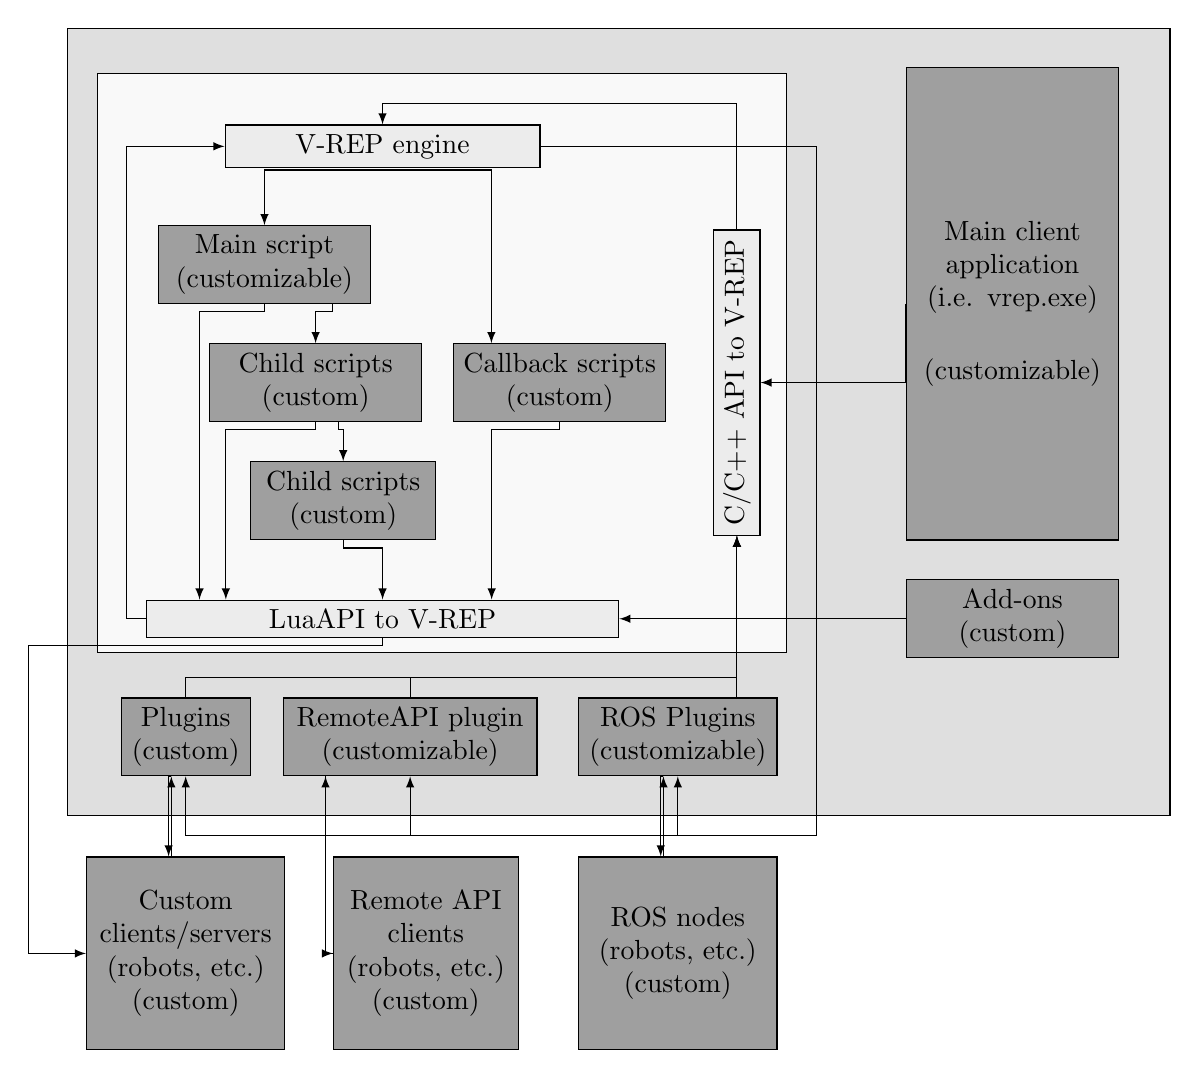
\begin{tikzpicture}
		\node (frameWork) at (0,0) [draw, rectangle, minimum width=14cm, minimum height=10cm, text 
		centered, fill=gray!25]{};
		
		\node (shareLibrary) at (-2.25,0.75) [draw, rectangle, minimum width=8.75cm, minimum 
		height=7.35cm, text centered, fill=gray!5]{};
		
		\node (V-REP engine) at (-3,3.5) [draw, rectangle, text centered, minimum width=4cm, 
		fill=gray!15]{V-REP engine};
		
		\node (Main Script) at (-4.5,2) [draw, rectangle, text centered, text width=7em, 
		fill=gray!75]{Main script\\(customizable)};
		
		\node (Child Script) at (-3.85,0.5) [draw, rectangle, text centered, text width=7em, 
		fill=gray!75]{Child scripts\\(custom)};
		
		\node (Callback Script) at (-0.75,0.5) [draw, rectangle, text centered, text width=7em, 
		fill=gray!75]{Callback scripts\\(custom)};
		
		\node (C/C++ API to V-REP) at (1.5,0.5) [draw, rectangle, rotate=90, text centered, 
		fill=gray!15]{C/C++ API to V-REP};
		
		\node (Child scripts2) at (-3.5,-1) [draw, rectangle, text centered, text width=6em, 
		fill=gray!75]{Child scripts\\(custom)};
		
		\node (LuaAPI) at (-3,-2.5) [draw, rectangle, text centered, minimum width=6cm, 
		fill=gray!15]{LuaAPI to V-REP};
		
		\node (Plugins) at (-5.5,-4) [draw, rectangle, text centered, text width=4em, 
		fill=gray!75]{Plugins\\(custom)};
		
		\node (RemoteAPI Plugins) at (-2.65,-4) [draw, rectangle, text centered, text width=8.5em, 
		fill=gray!75]{RemoteAPI plugin\\(customizable)};
		
		\node (ROS Plugins) at (0.75,-4) [draw, rectangle, text centered, text width=6.5em, 
		fill=gray!75]{ROS Plugins\\(customizable)};
		
		\node (Custom) at (-5.5,-6.75) [text centered, draw, rectangle, text width=6.5em, minimum 
		height=2.45cm, fill=gray!75]{Custom\\clients/servers\\(robots, etc.)\\(custom)};
		
		\node (Remote) at (-2.45,-6.75) [text centered, draw, rectangle, text width=6em, minimum 
		height=2.45cm, fill=gray!75]{Remote API\\clients\\(robots, etc.)\\(custom)};
		
		\node (ROSnodes) at (0.75,-6.75) [text centered, draw, rectangle, text width=6.5em, minimum 
		height=2.45cm, fill=gray!75]{ROS nodes\\(robots, etc.)\\(custom)};
		
		\node (Add-ons) at (5,-2.5) [draw, rectangle, text centered, text width=7em, 
		fill=gray!75]{Add-ons\\(custom)};
		
		\node (Main client) at (5,1.5) [draw, minimum height=6cm, rectangle, text centered, text 
		width=7em, fill=gray!75]{Main client\\application\\(i.e. 
		vrep.exe)\\\vspace{0.5cm}(customizable)};
		
		%Links
		\draw[-latex] (V-REP engine) ++(0,-0.3) -| (Main Script.90);
		\draw[-latex] (V-REP engine) ++(0,-0.3) -| (Callback Script.150);
		\draw[-latex] (V-REP engine.0) ++(0,0) -| ++(3.5,0) |- ++(0,-8.75) |- ++(0,0) -| (ROS 
		Plugins.270);
		\draw[-latex] (V-REP engine.0) ++(0,0) -| ++(3.5,0) |- ++(0,-8.75) |- ++(0,0) -| 
		(Plugins.270);
		\draw[-latex] (V-REP engine.0) ++(0,0) -| ++(3.5,0) |- ++(0,-8.75) |- ++(0,0) -| (RemoteAPI 
		Plugins.270);
		\draw[-latex] (LuaAPI.180) -| ++(-0.25,0) -| ++(0,0) |- (V-REP engine.180);
		\draw[-latex] (Main Script.330) ++(0,0) -| ++(0,-0.1) -| (Child Script.90);
		\draw[-latex] (Main Script.270) ++(0,0) -| ++(0,-0.1) -| (LuaAPI.174);
		\draw[-latex] (Child Script.270) ++(0,0) -| ++(0,-0.1) -| (LuaAPI.173);
		\draw[-latex] (Child Script.300) ++(0,0) -| ++(0,-0.1) -| (Child scripts2.90);
		\draw[-latex] (Child scripts2.270) ++(0,0) -| ++(0,-0.1) -| (LuaAPI.90);
		\draw[-latex] (Callback Script.270) ++(0,0) -| ++(0,-0.1) -| (LuaAPI.10);
		\draw[-latex] (Add-ons) -- (LuaAPI.0);
		\draw[-latex] (C/C++ API to V-REP.0) ++(0,0) |- ++(0,1.6) -| (V-REP engine.90);
		\draw[-latex] (Main client.180) ++(0,0) |- (C/C++ API to V-REP.270);
		\draw[-latex] (ROS Plugins.90) ++(0,0) -| ++(0,0) |- ++(0,0) |- ++(0,0) -| (C/C++ API to 
		V-REP.180);
		\draw[-latex] (RemoteAPI Plugins.90) ++(0,0) -| ++(0,0.25) |- ++(0,0) -| (C/C++ API to 
		V-REP.180);
		\draw[-latex] (Plugins.90) ++(0,0) -| ++(0,0.25) |- ++(0,0) -| (C/C++ API to V-REP.180);
		\draw[-latex] (ROSnodes.100) -| (ROS Plugins.250);
		\draw[latex-] (ROSnodes.100) |- (ROS Plugins.250);
		\draw[-latex] (Custom.100) -| (Plugins.250);
		\draw[latex-] (Custom.100) |- (Plugins.250);
		\draw[-latex] (LuaAPI.270) ++(0,0) -| ++(0,-0.1) |- ++(0,0) |- ++(-4.5,0) -| ++(0,0) |- 
		(Custom.180);
		\draw[-latex] (Remote.180) ++(0,0) |- ++(-0.1,0) -| (RemoteAPI Plugins.205);  
		\draw[-latex] (RemoteAPI Plugins.205) ++(0,0) |- (Remote.180);
		
		\end{tikzpicture}
	}
	\end{center}

\end{figure}

\section{Example \thevarious}
\stepcounter{various}

\begin{figure}[h]
	\centering
	\scalebox{0.4}{
		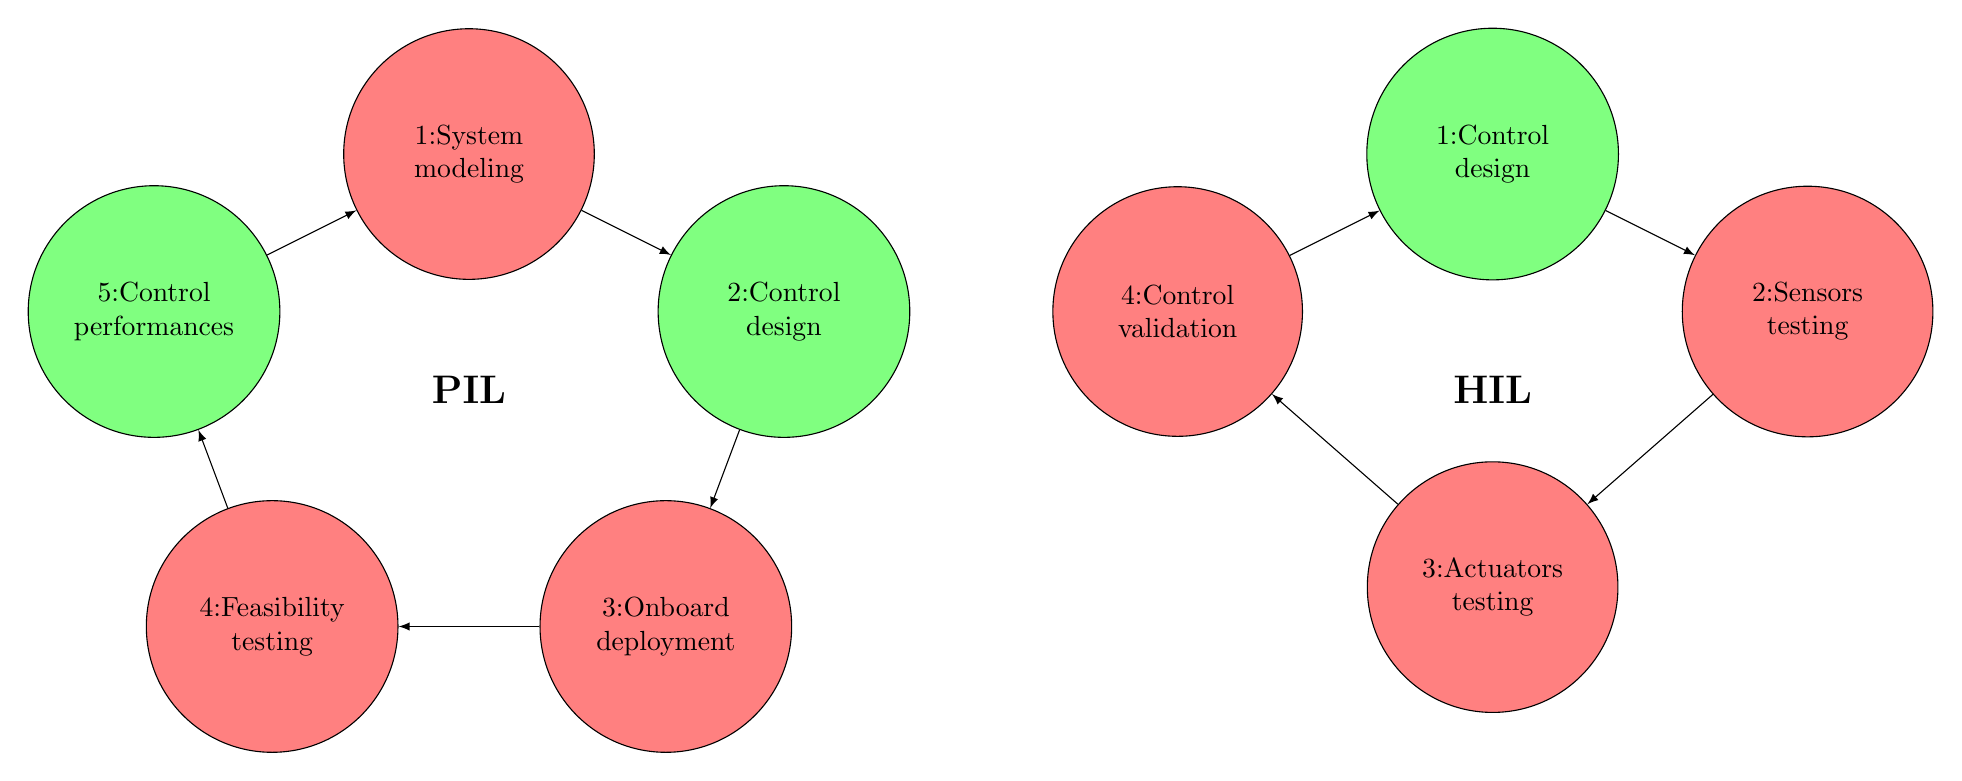
\begin{tikzpicture}
		%PIL's nodes
		\node (System Modeling) at (0,1) [circle, draw, minimum size=1cm, text centered, text 
		width=8em, fill=red!50]{1:System \\ modeling};
		\node (Control Design) at (4,-1) [circle, draw, minimum size=1cm, text centered, text 
		width=8em, fill=green!50]{2:Control \\ design};
		\node (Board Deploy) at (2.5,-5) [circle, draw, minimum size=1cm, text centered, text 
		width=8em, fill=red!50]{3:Onboard \\ deployment};
		
		\node (Feasibility Testing) at (-2.5,-5) [circle, draw, minimum size=1cm, text centered, 
		text width=8em, fill=red!50]{4:Feasibility \\ testing};
		\node (Control Performance) at (-4,-1) [circle, draw, minimum size=1cm, text centered, text 
		width=8em, fill=green!50]{5:Control \\ performances};
		
		\node (PIL) at (0,-2) [text centered]{\textbf{\Large{PIL}}};
		
		%PIL links
		\draw[-latex] (System Modeling) -- (Control Design);
		\draw[-latex] (Control Design) -- (Board Deploy);
		\draw[-latex] (Board Deploy) -- (Feasibility Testing);
		\draw[-latex] (Feasibility Testing) -- (Control Performance);
		\draw[-latex] (Control Performance) -- (System Modeling);
		
		%HIL's nodes
		\node (Control Design 1) at (13,1) [circle, draw, minimum size=1cm, text centered, text 
		width=8em, fill=green!50]{1:Control \\ design};
		\node (Sensor Testing) at (17,-1) [circle, draw, minimum size=1cm, text centered,  text 
		width=8em, fill=red!50]{2:Sensors \\ testing};
		\node (Actuators Testing) at (13,-4.5) [circle, draw, minimum size=1cm, text centered,  
		text width=8em, fill=red!50]{3:Actuators \\testing};
		\node (Control Validation) at (9,-1) [circle, draw, minimum size=1cm, text centered, text 
		width=8em, fill=red!50]{4:Control \\validation};
		
		\node (HIL) at (13,-2) [text centered]{\textbf{\Large{HIL}}};
		
		%HIL links
		\draw[-latex] (Control Design 1) -- (Sensor Testing);
		\draw[-latex] (Sensor Testing) -- (Actuators Testing);
		\draw[-latex] (Actuators Testing) -- (Control Validation);
		\draw[-latex] (Control Validation) -- (Control Design 1);
		
		\end{tikzpicture}
	}

\end{figure}

\newpage

\section{Example \thevarious}
\stepcounter{various}

\begin{figure}[h]
	\centering
	\subfigure[]{
		\scalebox{0.8}{
		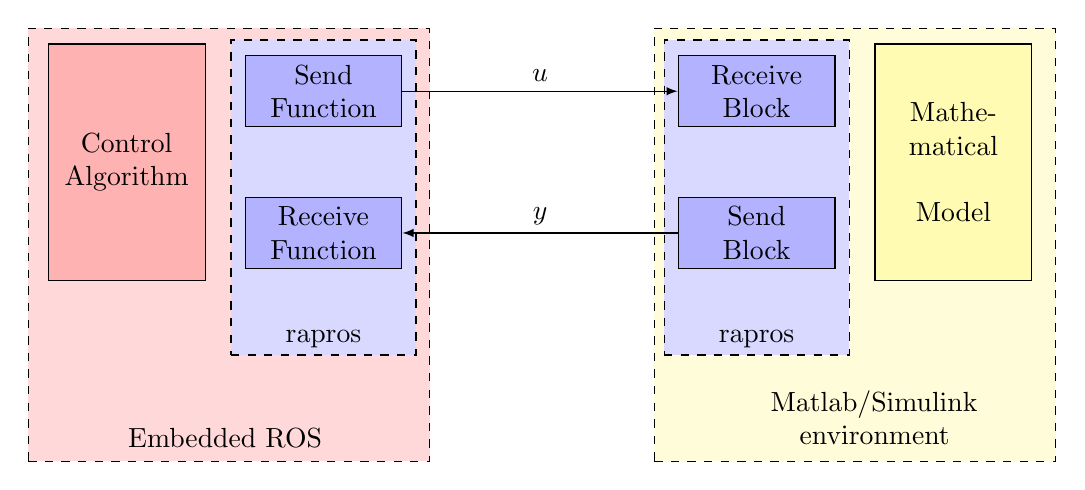
\begin{tikzpicture}
		%First block's components
		\node (Embedded ROS) at (0.05,-1.05) [draw, rectangle, dashed, minimum height=5.5cm, 
		minimum width=5.1cm, text centered, fill=red!15]{};
		\node (Control Algorithm) at (-1.25,0) [draw, rectangle, minimum height=3cm, minimum 
		width=1cm, text centered, text width=5em, fill=red!30]{Control \\Algorithm};
		\node (wrapper1) at (1.25,-0.45) [draw, rectangle, dashed, minimum height=4cm, minimum 
		width=2.35cm, text centered, fill=blue!15]{};
		\node (Send Function) at (1.25,0.9) [draw, rectangle, minimum height=0.5cm, minimum 
		width=1cm, text centered, text width=5em, fill=blue!30]{Send \\Function};
		\node (Receive Function) at (1.25,-0.9) [draw, rectangle, minimum height=0.5cm, minimum 
		width=1cm, text centered, text width=5em, fill=blue!30]{Receive \\Function};
		
		%Writing inside the first block
		\node (Scritto1) at (0,-3.5) [text centered]{Embedded ROS};
		\node (Scritto2) at (1.25,-2.25) [text centered]{rapros};
		
		%Second block's components
		\node (Embedded ROS) at (8,-1.05) [draw, rectangle, dashed, minimum height=5.5cm, minimum 
		width=5.1cm, text centered, fill=yellow!15]{};
		\node (Mathematical Model) at (9.25,0) [draw, rectangle, minimum height=3cm, minimum 
		width=1cm, text centered, text width=5em, fill=yellow!30]{Mathe-\\matical\\~\\Model};
		\node (wrapper1) at (6.75,-0.45) [draw, rectangle, dashed, minimum height=4cm, minimum 
		width=2.35cm, text centered, fill=blue!15]{};
		\node (Receive Block) at (6.75,0.9) [draw, rectangle, minimum height=0.5cm, minimum 
		width=1cm, text centered, text width=5em, fill=blue!30]{Receive \\Block};
		\node (Send Block) at (6.75,-0.9) [draw, rectangle, minimum height=0.5cm, minimum 
		width=1cm, text centered, text width=5em, fill=blue!30]{Send \\Block};
		
		%Writing inside the second block
		\node (Scritto1) at (8.25,-3.25) [text centered, text 
		width=9em]{Matlab/Simulink\textsuperscript{\circledR} \\environment};
		\node (Scritto2) at (6.75,-2.25) [text centered]{rapros};
		
		%Links amonb blocks
		\draw[-latex] (Send Function.0) -- (Receive Block.180) node at(4,1.3) [below]{$u$};
		\draw[-latex] (Send Block.180) -- (Receive Function.0) node at(4,-0.45) [below]{$y$};
		
		\end{tikzpicture}
	}
		
	}
	\subfigure[]{
		\scalebox{0.8}{
		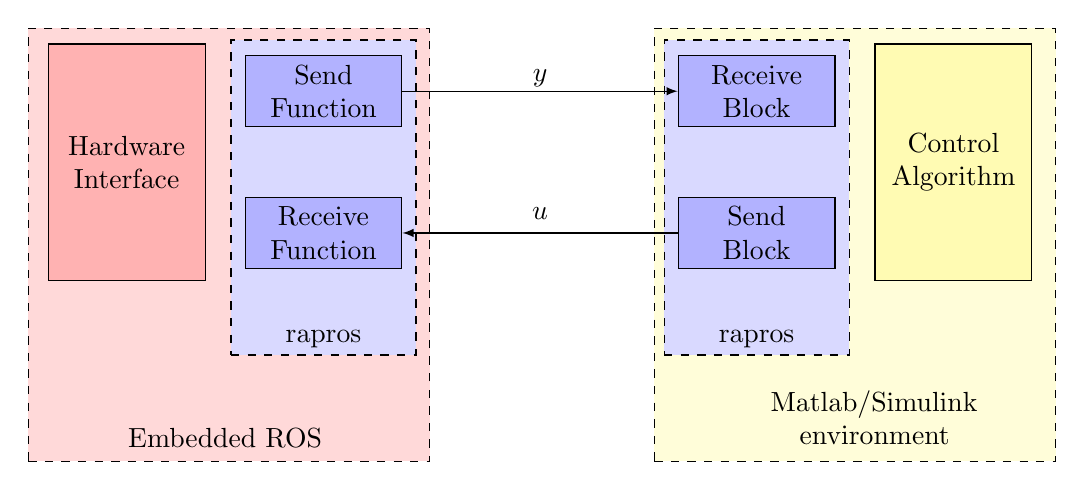
\begin{tikzpicture}
		\node (Embedded ROS) at (0.05,-1.05) [draw, rectangle, dashed, minimum height=5.5cm, 
		minimum width=5.1cm, text centered, fill=red!15]{};
		\node (Hardware Interface) at (-1.25,0) [draw, rectangle, minimum height=3cm, minimum 
		width=1cm, text centered, text width=5em, fill=red!30]{Hardware \\Interface};
		\node (wrapper1) at (1.25,-0.45) [draw, rectangle, dashed, minimum height=4cm, minimum 
		width=2.35cm, text centered, fill=blue!15]{};
		\node (Send Function) at (1.25,0.9) [draw, rectangle, minimum height=0.5cm, minimum 
		width=1cm, text centered, text width=5em, fill=blue!30]{Send \\Function};
		\node (Receive Function) at (1.25,-0.9) [draw, rectangle, minimum height=0.5cm, minimum 
		width=1cm, text centered, text width=5em, fill=blue!30]{Receive \\Function};
		
		\node (Scritto1) at (0,-3.5) [text centered]{Embedded ROS};
		\node (Scritto2) at (1.25,-2.25) [text centered]{rapros};
		
		\node (Embedded ROS) at (8,-1.05) [draw, rectangle, dashed, minimum height=5.5cm, minimum 
		width=5.1cm, text centered, fill=yellow!15]{};
		\node (Control Algorithm) at (9.25,0) [draw, rectangle, minimum height=3cm, minimum 
		width=1cm, text centered, text width=5em, fill=yellow!30]{Control\\Algorithm};
		\node (wrapper1) at (6.75,-0.45) [draw, rectangle, dashed, minimum height=4cm, minimum 
		width=2.35cm, text centered, fill=blue!15]{};
		\node (Receive Block) at (6.75,0.9) [draw, rectangle, minimum height=0.5cm, minimum 
		width=1cm, text centered, text width=5em, fill=blue!30]{Receive \\Block};
		\node (Send Block) at (6.75,-0.9) [draw, rectangle, minimum height=0.5cm, minimum 
		width=1cm, text centered, text width=5em, fill=blue!30]{Send \\Block};
		
		\node (Scritto1) at (8.25,-3.25) [text centered, text 
		width=9em]{Matlab/Simulink\textsuperscript{\circledR} \\environment};
		\node (Scritto2) at (6.75,-2.25) [text centered]{rapros};
		
		\draw[-latex] (Send Function.0) -- (Receive Block.180) node at(4,1.3) [below]{$y$};
		\draw[-latex] (Send Block.180) -- (Receive Function.0) node at(4,-0.45) [below]{$u$};
		\end{tikzpicture}
	}
		
	}

\end{figure}


\section{Example \thevarious}
\stepcounter{various}


\begin{figure}[h]
	\begin{center}
		\scalebox{0.8}{
		\begin{tikzpicture}
		
		%Reference system
		\draw[dashed] (-2,-2.75) coordinate -- (-2,0.75) coordinate;
		\draw[dashed] (-2,-3.25) coordinate -- (-2,-3.5) coordinate;
		
		%First sphere
		\node (firstSphere) at(0,0) [draw, circle, minimum size=0.5cm, text centered, left 
		color=gray!50, right color=white, shading = axis]{};
		\draw (0.25,0) node[right]{$m,\,I$};
		
		%Body
		\filldraw[left color=gray!50, right color=white, shading = axis] (-4,-3) rectangle (0,-5);
		
		%Second sphere
		\node (secondSphere) at(-2,-3) [draw, circle, left color=gray!50, right color=white, 
		shading = axis, minimum size=0.15cm, text centered]{};
		
		%Links
		\draw[line width=1.25pt] (firstSphere) -- (secondSphere);
		\draw (-0.75,-1.7) node{$l$};
		
		%Arrow
		\draw[-latex, line width=1.25pt] (-5,-4) node[above right]{$F$} -- (-4,-4);
		
		%Angle
		\draw[] (secondSphere) -- (0,-3) coordinate (c);
		\draw pic["$\mathbf{\theta}$", draw, -latex, angle eccentricity=1.2, angle 
		radius=1cm]{angle=c--secondSphere--firstSphere};
		
		%Wheels
		\node (firstWheel) at(-3,-5.25) [draw, circle, left color=gray!50, right color=white, 
		shading = axis, minimum size=0.75cm, text centered]{};
		\node (secondWheel) at(-1,-5.25) [draw, circle, left color=gray!50, right color=white, 
		shading = axis, minimum size=0.75cm, text centered]{};
		
		%Baseline
		\draw[line width=1.25pt] (-5,-5.65) coordinate -- (1,-5.65) coordinate;
		
		%x
		\draw[-latex, line width=1.25pt] (0,-5.35) coordinate -- (1,-5.35) coordinate node[above 
		left]{$x$};
		
		%body mass
		\draw (-2,-3.75) coordinate node[below]{$M$};
		
		\end{tikzpicture}
	}
	\end{center}
\end{figure}

\newpage


\section{Example \thevarious}
\stepcounter{various}

\begin{figure}[h]
	\begin{center}
		\begin{tikzpicture}
		
		%Reference system
		\draw[dashed] (-2,-2.75) coordinate -- (-2,0.75) coordinate;
		\draw[dashed] (-2,-3.25) coordinate -- (-2,-3.5) coordinate;
		
		%First sphere
		\node (firstSphere) at(0,0) [draw, circle, minimum size=0.5cm, text centered, left 
		color=gray!50, right color=white, shading = axis]{};
		\draw (0.25,0) node[right]{$m,\,I$};
		
		%Body
		\filldraw[left color=gray!50, right color=white, shading = axis] (-4,-3) rectangle (0,-5);
		
		%Second sphere
		\node (secondSphere) at(-2,-3) [draw, circle, left color=gray!50, right color=white, 
		shading = axis, minimum size=0.15cm, text centered]{};
		
		%Links
		\draw[line width=1.25pt] (firstSphere) -- (secondSphere);
		\draw (-0.75,-1.7) node{$l$};
		
		%Arrow
		\draw[-latex, red, line width=1.25pt] (-5,-4) node[above right]{$F$} -- (-4,-4);
		
		%Frction force
		\draw[latex-, red, line width=1.25pt] (0,-4) coordinate node[above right]{$friction$} -- 
		(1,-4) coordinate node[below]{$=b\dot{x}$};
		
		%Forces
		\draw[-latex, red, line width=1.25pt] (-2,-3) coordinate -- (-2,-4) coordinate 
		node[left]{$P$};
		\draw[-latex, red, line width=1.25pt] (-2,-3) coordinate -- (-3,-3) coordinate 
		node[above]{$N$};
		
		\draw[-latex, red, line width=1.25pt] (-1.75,-2.75) coordinate -- (-1.75,-1.5) coordinate;
		\draw[-latex, red, line width=1.25pt] (-1.75,-2.75) coordinate -- (-0.5,-2.75) coordinate 
		node[above]{$N$};
		
		\draw[-latex, red, line width=1.25pt] (-0.4,-0.65) coordinate -- (-0.4,-1.65) coordinate 
		node[above right]{$mg$};
		
		%Angle
		\draw[] (secondSphere) -- (0,-3) coordinate (c);
		\draw pic["$\mathbf{\theta}$", draw, -latex, angle eccentricity=1.2, angle 
		radius=1cm]{angle=c--secondSphere--firstSphere};
		
		%Wheels
		\node (firstWheel) at(-3,-5.25) [draw, circle, left color=gray!50, right color=white, 
		shading = axis, minimum size=0.75cm, text centered]{};
		\node (secondWheel) at(-1,-5.25) [draw, circle, left color=gray!50, right color=white, 
		shading = axis, minimum size=0.75cm, text centered]{};
		
		%Baseline
		\draw[line width=1.25pt] (-5,-5.65) coordinate -- (1,-5.65) coordinate;
		
		%X
		\draw[-latex, line width=1.25pt] (0,-5.35) coordinate -- (1,-5.35) coordinate node[above 
		left]{$x$};
		
		\end{tikzpicture}
	\end{center}

\end{figure}


\section{Example \thevarious}
\stepcounter{various}

\begin{figure}[h]
	\begin{center}
		\begin{tikzpicture}
		
		%Virtual reference system 
		\draw[latex-] (0.4,2) [draw=green] arc (0:-90:1.2cm) node[anchor=south]{$\phi$};
		
		\draw[latex-] (2.7,0.6) [draw=yellow] arc (0:-130:1cm)  node[anchor=north]{$\psi$};
		
		\draw[latex-] (-0.6,-0.7) [draw=red] arc (0:-140:1cm) node[anchor=east]{$\theta$};
		
		%Real reference system
		\draw[-latex] (0,0) coordinate (Creal) node[anchor=east]{$C_{dr}$} -- (3,0) coordinate 
		(Zreale) node[anchor=west] {$X_{dr}$};
		
		\draw[-latex] (0,-3) coordinate (NegYreal) -- (0,3) coordinate (Yreale) node[anchor=south] 
		{$Z_{dr}$};
		
		\draw[-latex] (-2.0,-2.0) node[anchor=east]{$-Y_{dr}$} -- (1.5,1.5) coordinate (Xreal) 
		node[anchor=west] {$Y_{dr}$};
		
		%Angles virtual reference system
		\draw[latex-] (7,2) [draw=green] arc (0:-90:1.2cm) node[anchor=south]{$\theta$};
		
		\draw[latex-] (9.3,0.6) [draw=yellow] arc (0:-130:1cm)  node[anchor=north]{$\phi$};
		
		\draw[latex-] (6.0,-0.7) [draw=red] arc (0:-140:1cm) node[anchor=east]{$\psi$};
		
		%Virtual reference system		
		\draw[-latex] (6.6,0) coordinate (Cvirtual) node[anchor=east]{$C_{vr}$} -- (9.6,0) 
		coordinate (Yvirtuale) node[anchor=west] {$X_{vr}$};
		
		\draw[-latex] (6.6,-3) coordinate (NegZvirtual) -- (6.6,3) coordinate (Zvirtual) 
		node[anchor=south] {$Y_{vr}$};
		
		\draw[latex-] (4.6,-2.0) node[anchor=east]{$Z_{vr}$} -- (8.1,1.5) coordinate (Xvirtual) 
		node[anchor=west] {$-Z_{vr}$};
		
		\end{tikzpicture}
	\end{center}
	
\end{figure}

\newpage

\section{Example \thevarious}
\stepcounter{various}

\begin{figure}[h]
	\begin{center}
		\scalebox{1}{
			\begin{tikzpicture}
			
			%Bounding box
			\node (boundingBox) at (0,0) [rectangle, draw, minimum width=10cm, minimum height=4cm, 
			text centered, label=\textbf{Frame}]{};
			
			%Vertices coordinates
			\node (verticesCoordinates) at (-5,2) [circle, draw, scale=0.4, fill=black]{}; 
			\draw (-5,2) coordinate node[above left]{$(x_0,\,y_0)$};
			
			%Curly brackets
			\draw [decorate,decoration={brace,amplitude=10pt,raise=4pt},yshift=0pt]
			(5,2) -- (5,-2) node [black,midway,xshift=1.1cm] {\footnotesize
			$h_{\mathrm{img}}$};
			
			\draw [decorate,decoration={brace,mirror,amplitude=10pt,raise=4pt},yshift=0pt]
			(-5,-2) -- (5,-2) node [black,midway,xshift=0cm, yshift=-0.75cm] {\footnotesize
			$w_{\mathrm{img}}$};
			
			%Curcly brackets bounding box
			\draw [decorate,decoration={brace,mirror,amplitude=10pt,raise=4pt},yshift=0pt]
			(-0.9,-1.825) -- (-0.9,-0.575) node [black,midway,xshift=1cm] {\footnotesize
			$h_{bb}$};
			
			\draw [decorate,decoration={brace, amplitude=10pt,raise=4pt},yshift=0pt]
			(-4.3,-0.50) -- (-0.9,-0.50) node [black,midway,xshift=0cm, yshift=0.75cm] 
			{\footnotesize	$w_{bb}$};
			
			%Image centroid coordinates
			\draw[dashed,draw=blue] (0,0) coordinate -- (0,2) coordinate;
			\draw[dashed,draw=blue] (0,0) coordinate -- (5,0) coordinate;
			\node (nomeCentroideImg) at (0,0) [circle, draw, scale=0.4, fill=black]{};
			\draw (0,0) coordinate node[below right]{$(x_{\mathrm{img}},\,y_{\mathrm{img}})$};
			
			%Centroids
			\node (nameCentroidBB) at (-2.6,-1.2) [circle, draw, scale=0.5, fill=black]{};
			\draw (-2.6,-1.5) coordinate node[above left]{$(x_{bb},\,y_{bb})$};
			
			%Bounding box sorrounding the target
			\node (bb) at (-2.6, -1.2) [rectangle, draw=red, minimum width=3.4cm, minimum 
			height=1.25cm, dashed]{}; 
			
			%Vector among centroids
			\draw[-latex, draw=green] (0,0) coordinate -- (-2.6,-1.2) coordinate; 
			
			%Reference syste,
			\draw[-latex] (-6.7,3.2) coordinate -- (-6.7,-3.2) coordinate node[above left]{$y$};
			\draw[-latex] (-6.7,3.2) coordinate -- (6.7,3.2) coordinate node[below right]{$x$}; 
			
			\end{tikzpicture}
		}
	\end{center}
	
\end{figure}


\section{Example \thevarious}
\stepcounter{various}

\begin{figure}[h]
	\begin{center}
	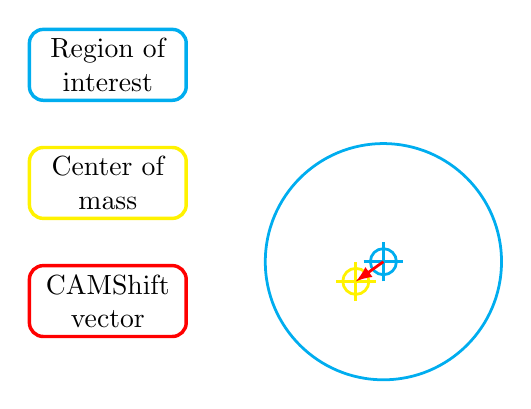
\begin{tikzpicture}
	
	\pgfmathsetseed{2};
	%Features inside the ROI
	\fillrandomly{2}{2}{0.1}{100};
	\node at (1,1) [circle, line width=1.0pt, draw=cyan, text centered, minimum size=3cm]{};
	%Features outside the ROI
	\fillrandomly{6}{3}{0.1}{50};
	
	%Legend
	\node at (-2.5,3.5) [draw, rectangle, line width=1.25pt, rounded corners=5pt, text width=5em, 
	draw=cyan, text centered]{Region of \\interest};
	\node at (-2.5,2) [draw, rectangle, line width=1.25pt, rounded corners=5pt, text width=5em, 
	draw=yellow, text centered]{Center of \\mass};
	\node at (-2.5,0.5) [draw, rectangle, line width=1.25pt, rounded corners=5pt, text width=5em, 
	draw=red, text centered]{CAMShift \\vector};
	
	\node at (1,1) [circle, line width=1.0pt, draw=cyan, text centered]{};
	\draw[-, cyan, line width=1.0pt] (1,0.75) coordinate -- (1,1.25) coordinate;
	\draw[-, cyan, line width=1.0pt] (0.75,1) coordinate -- (1.25,1) coordinate;
	
	\node at (0.65,0.75) [circle, line width=1.0pt, draw=yellow, text centered]{};
	\draw[-, yellow, line width=1.0pt] (0.65,0.5) coordinate -- (0.65,1.0) coordinate;
	\draw[-, yellow, line width=1.0pt] (0.40,0.75) coordinate -- (0.90,0.75) coordinate;
	\draw[-latex, red, line width=1.0pt] (1,1) coordinate -- (0.65,0.75) coordinate;
	
	\end{tikzpicture}
	\end{center}
\end{figure}

\newpage

\section{Example \thevarious}
\stepcounter{various}

\begin{figure}[h]
	\begin{center}
		\scalebox{0.8}{
			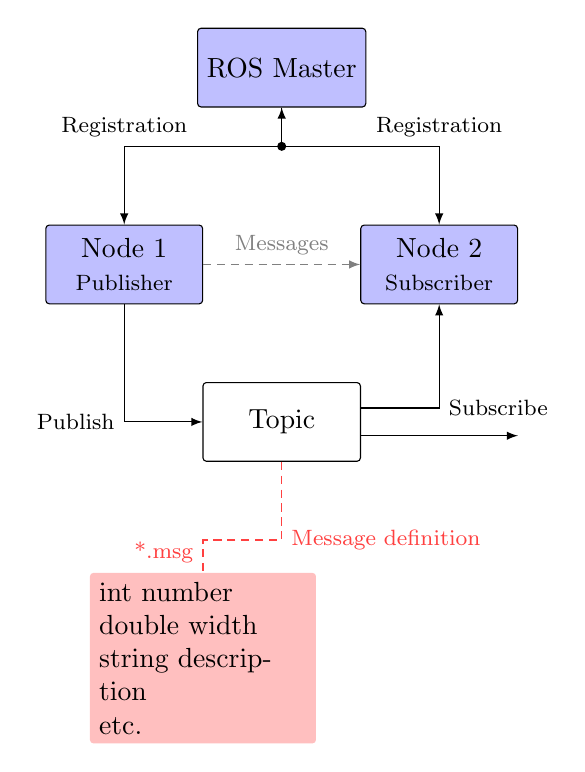
\begin{tikzpicture}
			
			%Nodes
			\node (ROSMaster) at (0,1) [rectangle, draw, minimum height=1cm, minimum width=1cm, 
			rounded corners=1.25pt, text centered, fill={blue!25}]{ROS Master};
			\node (Node1) at (-2,-1.5) [rectangle, draw, minimum height=1cm, minimum width=1cm, 
			rounded corners=1.25pt, text centered, text width=5em, fill={blue!25}]{Node 
			1\\\footnotesize{Publisher}};
			\node (Node2) at (2,-1.5) [rectangle, draw, minimum height=1cm, minimum width=1cm, 
			rounded corners=1.25pt, text centered, text width=5em, fill={blue!25}]{Node 
			2\\\footnotesize{Subscriber}};
			\node (Topic) at (0,-3.5) [rectangle, draw, minimum height=1cm, minimum width=2cm, 
			rounded corners=1.25pt, text centered]{Topic};
			
			
			%Messages
			\node (StrutturaMessaggio) at (-1,-6.5) [rectangle,minimum height=1cm, minimum 
			width=2cm, fill={red!25}, rounded corners=1.25pt, text width=7.5em]{int number\\double 
			width\\string description\\etc.};
			
			%Links
			\draw[latex-latex] (ROSMaster) -- (0,0) coordinate -| 
			node[above]{\footnotesize{Registration}} (Node1);
			\draw[-latex] (ROSMaster) -- (0,0) coordinate -| 
			node[above]{\footnotesize{Registration}} (Node2);
			\draw[-latex, gray, densely dashed] (Node1) -- node[above]{\footnotesize{Messages}} 
			(Node2);
			\draw[-latex] (Node1) |- node[left]{\footnotesize{Publish}}(Topic);
			\draw[-latex] (Topic.10) -| node[right]{\footnotesize{Subscribe}}(Node2);
			\draw[-latex] (1,-3.675) -- (3,-3.675) coordinate;
			\draw[densely dashed, red!75, text=red!75] (Topic.south) -- (0,-5) coordinate 
			node[right]{\footnotesize{Message definition}} -| (StrutturaMessaggio.north) node[above 
			left]{\footnotesize{*.msg}};
			
			%Bubbles
			\node (bubble1) at (0,0) [circle, draw, scale=0.3, fill=black]{};
			
			\end{tikzpicture}
		}
	\end{center}
\end{figure}

\section{Example \thevarious}
\stepcounter{various}

\begin{figure}[h]
	\begin{center}
		\scalebox{0.8}{
			\begin{forest}
				for tree={
					font=\sffamily,
					rounded corners=4pt,
					grow'=0,
					inner ysep=8pt,
					child anchor=west,
					parent anchor=south,
					anchor=west,
					calign=first,
					edge={rounded corners},
					edge path={
						\noexpand\path [draw, \forestoption{edge}]
						(!u.south west) +(12.5pt,0) |- (.child anchor)\forestoption{edge label};
					},
					before typesetting nodes={
						if n=1
						{insert before={[,phantom,minimum height=18pt]}}
						{}
					},
					fit=band,
					s sep=12pt,
					before computing xy={l=25pt},
				}
				[\myfolder{pkg}
				[\myfolder{config}]
				[\myfolder{include}
				[{\myfolder{pkg}}]
				]
				[\myfolder{launch}]
				[\myfolder{src}]
				[\myfolder{test}]
				[]
				]
			\end{forest}
		}
	\end{center}
\end{figure}

\newpage

\section{Example \thevarious}
\stepcounter{various}

	
\begin{figure}[h]
	\begin{center}
		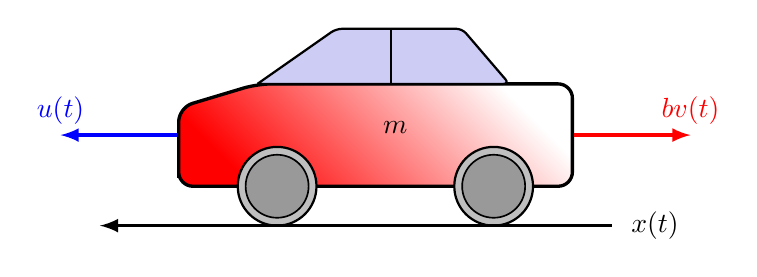
\begin{tikzpicture}
		\shade[top color=red, bottom color=white, shading angle={135}]
		[draw=black,fill=red!20,rounded corners=1.2ex,very thick] (1.5,.5) -- ++(0,1) -- ++(1,0.3) 
		--  ++(3,0) -- ++(1,0) -- ++(0,-1.3) -- (1.5,.5) -- cycle;
		\draw[very thick, rounded corners=0.5ex,fill=black!20!blue!20!white,thick]  (2.5,1.8) -- 
		++(1,0.7) -- ++(1.6,0) -- ++(0.6,-0.7) -- (2.5,1.8);
		\draw[thick]  (4.2,1.8) -- (4.2,2.5);
		\draw[draw=black,fill=gray!50,thick] (2.75,.5) circle (.5);
		\draw[draw=black,fill=gray!50,thick] (5.5,.5) circle (.5);
		\draw[draw=black,fill=gray!80,semithick] (2.75,.5) circle (.4);
		\draw[draw=black,fill=gray!80,semithick] (5.5,.5) circle (.4);
		
		\draw[latex-, semithick, line width=1.25pt] (.5,0) -- (7,0);
		\draw (7.55,0) node {$x(t)$};
		\draw (4.25,1.25) node {$m$};
		
		%Rappresento le forze
		\draw[-latex, red, line width=1.25pt] (6.52,1.15) coordinate --(8,1.15) coordinate 
		node[above]{$bv(t)$};
		\draw[latex-, blue, line width=1.25pt] (0,1.15) coordinate node[above]{$u(t)$} 
		--(1.48,1.15) coordinate;
		\end{tikzpicture}
	\end{center}
\end{figure}


\section{Example \thevarious}
\stepcounter{various}

\begin{figure}[h]
	\begin{center}
		\begin{tikzpicture}
		
		% Ground vehicle path
		\node (vertexGround1) at (0,0) [circle, scale=0.45, fill=black, draw]{};
		\node (vertexGround2) at (1,-3) [circle, scale=0.45, fill=black, draw]{};
		\node (vertexGround3) at (-1,-3.5) [circle, scale=0.45, fill=black, draw]{};
		\node (vertexGround4) at (-2.5,-2.5) [circle, scale=0.45, fill=black, draw]{};
		\node (vertexGround5) at (-2,-2.25) [circle, scale=0.45, fill=black, draw]{};
		
		% Linking the ground vehicle vertices
		\draw[blue] (vertexGround1) -- (vertexGround2);
		\draw[blue] (vertexGround2) -- (vertexGround3);
		\draw[blue] (vertexGround3) -- (vertexGround4);
		\draw[blue] (vertexGround4) -- (vertexGround5);
		\draw[blue] (vertexGround5) -- (vertexGround1);
		
		% UAV path
		\node (vertexUAV1) at (1.5,-3.75) [circle, scale=0.45, fill=black, draw]{};
		\node (vertexUAV2) at (1.5,-2.25) [circle, scale=0.45, fill=black, draw]{};
		\node (vertexUAV3) at (-1,-4.5) [circle, scale=0.45, fill=black, draw]{};
		
		\node (vertexUAV4) at (-1,1) [circle, scale=0.45, fill=black, draw]{};
		\node (vertexUAV5) at (0.5,1.5) [circle, scale=0.45, fill=black, draw]{};
		\node (vertexUAV6) at (-0.35,2) [circle, scale=0.45, fill=black, draw]{};
		
		% Linking the UAV vertices
		\draw[red] (vertexUAV1) -- (vertexUAV2);
		\draw[red] (vertexUAV2) -- (vertexGround2);
		\draw[red] (vertexUAV1) -- (vertexGround2);
		
		\draw[red] (vertexUAV3) -- (vertexGround3);
		
		\draw[red] (vertexUAV4) -- (vertexUAV5);
		\draw[red] (vertexUAV5) -- (vertexUAV6);
		\draw[red] (vertexUAV6) -- (vertexUAV4);
		
		% Ground vehicle path
		\node (vertexGround6) at (3,-1.5) [circle, scale=0.45, fill=black, draw]{};
		\node (vertexGround7) at (4,0) [circle, scale=0.45, fill=black, draw]{};
		\node (vertexGround8) at (4,-3) [circle, scale=0.45, fill=black, draw]{};
		
		\draw[blue] (vertexGround6) -- (vertexGround7);
		\draw[blue] (vertexGround7) -- (vertexGround8);
		\draw[blue] (vertexGround8) -- (vertexGround6);
		
		% UAV vertices
		\node (vertexUAV7) at (2.25,-1) [circle, scale=0.45, fill=black, draw]{};
		\draw[red] (vertexUAV7) -- (vertexGround6);
		
		% Legend
		\node (legend) at (7,0) [rectangle, draw, minimum width=2cm, text 
		width=8em]{\hspace{0.5cm}Targets\\\hspace{0.5cm}GV Path\\\hspace{0.5cm}UAV Path};
		\node at (5.7,0.5) [circle, scale=0.45, fill=black, draw]{};
		\draw[blue, line width=1.25pt] (5.55,0) -- (5.8,0);
		\draw[red, line width=1.25pt] (5.55,-0.45) -- (5.8,-0.45);
		
		\end{tikzpicture}
	\end{center}
\end{figure}